%!TEX TS-program =  pdflatex 


\documentclass{amsart}
\usepackage{array}
\newcolumntype{P}[1]{>{\raggedright\let\newline\\\arraybackslash\hspace{0pt}}m{#1}}
\usepackage{graphicx,verbatim, amsmath, amssymb, amsthm, amsfonts, epsfig, amsxtra,ifthen,mathtools,epstopdf,caption,enumerate,hyperref,hhline,bbm,capt-of,longtable}	
\DeclareFontFamily{U}{mathx}{\hyphenchar\font45}
\DeclareFontShape{U}{mathx}{m}{n}{<-> mathx10}{}
\DeclareSymbolFont{mathx}{U}{mathx}{m}{n}
\DeclareMathAccent{\widebar}{0}{mathx}{"73}
\epstopdfsetup{suffix=}
\DeclareGraphicsExtensions{.ps}
\DeclareGraphicsRule{.ps}{pdf}{.pdf}{`ps2pdf -dEPSCrop -dNOSAFER #1 \noexpand\OutputFile}

\newtheorem{proposition}{Proposition}[section]
\newtheorem{theorem}[proposition]{Theorem}
\newtheorem{corollary}[proposition]{Corollary}
\newtheorem{lemma}[proposition]{Lemma}
\newtheorem{prop}[proposition]{Proposition}
\newtheorem{cor}[proposition]{Corollary}
\newtheorem{thm}[proposition]{Theorem}
\newtheorem{conj}[proposition]{Conjecture}
\newtheorem{phen}{Phenomenon}

\renewcommand\thephen{\Roman{phen}}

\theoremstyle{definition}
\newtheorem{example}[proposition]{Example}
\newtheorem{definition}[proposition]{Definition}
\newtheorem{question}[proposition]{Question}

\theoremstyle{remark}
\newtheorem{remark}[proposition]{Remark}
\newtheorem{problem}[proposition]{Problem}

\numberwithin{equation}{section}
\usepackage[usenames]{color}

% commands for marginal notes below
% to make a marginal note, insert
% \margin{Your comment here.} in the text.
%  To sign the note:
% \margin[You]{Your comment here.}
% You can also label your comments and get a reference to the 
% number later, like:
% \margin[You]{Your comment here. \label{thefrivolouscomment}}
% Things may start to look ugly if you have more than 99 
%  marginal notes, but utility, not beauty is the intention here.
%  This uses the command \marginpar
%  defined, I think, in verbatim
%  The circled numbers will screw up the formatting slightly.

% Sometimes, if you terminate a run of LaTeX with "X" while using this macro, the next time you compile you will get the error "! File ended while scanning use of \@newl@bel.". The solution is to delete the .aux file (and fix whatever made you abort the run in the first place) and run LaTeX again.
% Another solution seems to be to terminate the new run with "q" and then run again.
\usepackage{color}

% to set color for comment numbers, use any of the 68 colors from 
% the color package in the command below
\newcommand{\margincolor}{red}      
\definecolor{darkgreen}{rgb}{0,0.7,0}
\newcommand{\marginauthorcolor}{darkgreen}      

% control the width of your comments
\addtolength{\marginparwidth}{8mm}

\newcounter{margincounter}
\setcounter{margincounter}{0}

\newcommand{\marginnum}{
\ifnum\value{margincounter}<10
\textcolor{\margincolor}{\begin{picture}(0,0)\put(2.2,2.4){\circle{9}}\end{picture}\footnotesize\arabic{margincounter}}
\else\ifnum\value{margincounter}<100
\textcolor{\margincolor}{\begin{picture}(0,0)\put(4.256,2.5){\circle{11}}\end{picture}\footnotesize\arabic{margincounter}}
\else
\textcolor{\margincolor}{\begin{picture}(0,0)\put(6.8,2.5){\circle{14}}\end{picture}\footnotesize\arabic{margincounter}}
\fi\fi
}

%\newcommand{\marginnum}{\textcolor{\margincolor}{\begin{picture}(0,0)\put(4.256,2.5){\circle{11}}\end{picture}\footnotesize\arabic{margincounter}}}


\newcommand{\margin}[2][]
{\!\!\refstepcounter{margincounter}\marginnum\marginpar{\textcolor{\margincolor}{\arabic{margincounter}.}\,\,\tiny #2\,\,\,\textcolor{\marginauthorcolor}{\small#1}}}
%  If you want to switch which margin you're using, do the command  \reversemarginpar before your marginal comment.
% To switch back, do \normalmarginpar
% (But I think it won't let you switch which margin you use in the middle of a paragraph of the main text.

%  to remove marginal notes, uncomment the following:
%  \renewcommand{\margin}[2][]{}
%  to remove just the circled numbers in the text, uncomment the following:
%  \renewcommand{\marginnum}{}
%  For final versions of a paper, it's probably best to remove all the \margin
%  commands.  Much to my annoyance, they mess up the typesetting.
\newcommand{\marginN}[1]{\margin[NR]{#1}}


% This is for setting off words we define in a separate typeface.
\newcommand{\newword}[1]{\textbf{\emph{#1}}}

\newcommand{\integers}{\mathbb Z}
\newcommand{\rationals}{\mathbb Q}
\newcommand{\naturals}{\mathbb N}
\newcommand{\reals}{\mathbb R}

\newcommand{\ep}{\varepsilon}
\newcommand{\thet}{\vartheta}
\newcommand{\col}{\mathbf{col}}
\newcommand{\id}{\operatorname{id}}
\newcommand{\cl}{\operatorname{cl}}
\newcommand{\cw}{\operatorname{cw}}
\newcommand{\ccw}{\operatorname{ccw}}
\newcommand{\sgn}{\operatorname{sgn}}
\newcommand{\vsgn}{\mathbf{sgn}}
\newcommand{\Seed}{\operatorname{Seed}}
\newcommand{\Sh}{{\mathcal Sh}}
\newcommand{\lcm}{\operatorname{lcm}}
\newcommand{\rank}{\operatorname{rank}}
\newcommand{\Int}{\operatorname{Int}}
\newcommand{\Fix}{\operatorname{Fix}}
\newcommand{\Stab}{\operatorname{Stab}}
\newcommand{\geom}{{\operatorname{geom}}}
\newcommand{\mon}{{\operatorname{mon}}}
\newcommand{\Ray}{{\operatorname{Ray}}}
\newcommand{\Ram}{{\operatorname{Ram}}}
\newcommand{\uf}{{\operatorname{uf}}}
\newcommand{\fr}{{\operatorname{fr}}}
\newcommand{\Geom}{{\operatorname{\textbf{Geom}}}}
\newcommand{\Cg}{\mbox{{\rm Cg}}}
\newcommand{\Con}{\mbox{{\rm Con}}}
\newcommand{\Irr}{\mbox{{\rm Irr}}}
\newcommand{\cov}{\mathrm{cov}}
\newcommand{\fs}{\mathrm{fs}}
\newcommand{\ufs}{\mathrm{ufs}}
\newcommand{\covers}{{\,\,\,\cdot\!\!\!\! >\,\,}}
\newcommand{\covered}{{\,\,<\!\!\!\!\cdot\,\,\,}}
\newcommand{\set}[1]{{\lbrace #1 \rbrace}}
\newcommand{\sett}[1]{{\bigl\lbrace #1 \bigr\rbrace}}
\newcommand{\settt}[1]{{\Bigl\lbrace #1 \Bigr\rbrace}}
\newcommand{\setttt}[1]{{\biggl\lbrace #1 \biggr\rbrace}}
\newcommand{\settttt}[1]{{\Biggl\lbrace #1 \Biggr\rbrace}}
\newcommand{\pidown}{\pi_\downarrow}
\newcommand{\piup}{\pi^\uparrow}
\newcommand{\br}[1]{{\langle #1 \rangle}}
\newcommand{\A}{{\mathcal A}}
\newcommand{\EL}{{\mathcal L}}
\newcommand{\F}{{\mathcal F}}
\newcommand{\D}{{\mathfrak D}}
\newcommand{\N}{{\mathcal N}}
\newcommand{\p}{{\mathfrak p}}
\newcommand{\X}{{\mathcal X}}
\newcommand{\W}{{\mathcal W}}
\newcommand{\join}{\vee}
\newcommand{\meet}{\wedge}
\renewcommand{\Join}{\bigvee}
\newcommand{\Meet}{\bigwedge}
\newcommand{\bigmeet}{\Meet}
\newcommand{\bigjoin}{\Join}
\newcommand{\leftq}[2]{\!\!\phantom{.}^{#1} {#2}}
\newcommand{\closeleftq}[2]{\!\!\phantom{.}^{#1}\! {#2}}
\newcommand{\Pge}{{\Phi_{\ge -1}}}
\newcommand{\cm}{\parallel}
%\newcommand{\ck}{^\vee}
%\newcommand{\ck}{^{\scalebox{0.5}[0.5]{$\vee$}}}
\newcommand{\ck}{\spcheck}
\newcommand{\letw}{\le_{\mathrm{tw}}}
\newcommand{\Alg}{\mathrm{Alg}}
\newcommand{\toname}[1]{\stackrel{#1}{\longrightarrow}}
\newcommand{\dashname}[1]{\stackrel{#1}{\mbox{---\!---}}}
\newcommand{\st}{^\mathrm{st}}
\renewcommand{\th}{^\text{th}}
\newcommand{\nd}{^\text{nd}}
\newcommand{\rd}{^\text{rd}}
\newcommand{\0}{{\mathbf{0}}}
\newcommand{\Vol}{\mathrm{Vol}}
\newcommand{\lleq}{\le\!\!\!\le}
\newcommand{\notlleq}{\le\!\!\!\!\not\,\le}
\newcommand{\ggeq}{\ge\!\!\!\ge}
\newcommand{\FF}{\mathcal{F}}
\newcommand{\ZZ}{\mathbb{Z}}
\newcommand{\QQ}{\mathbb{Q}}
\newcommand{\RR}{\mathbb{R}}
\newcommand{\CC}{\mathbb{C}}
\newcommand{\PP}{\mathbb{P}}
\newcommand{\GL}{\mathrm{GL}}
\newcommand{\Tits}{\mathrm{Tits}}
\newcommand{\Cone}{\mathrm{Cone}}
\newcommand{\Star}{\mathrm{Star}}
\newcommand{\Lin}{\mathrm{Lin}}
\newcommand{\Ker}{\mathrm{Ker}}
\newcommand{\Proj}{\mathrm{Proj}}
\newcommand{\relint}{\mathrm{relint}}
\newcommand{\Clust}{\mathrm{Clust}}
\newcommand{\into}{\hookrightarrow}
\newcommand{\equivalent}{\Longleftrightarrow}
\newcommand{\onto}{\twoheadrightarrow}
\newcommand{\isomorph}{\cong}
\newcommand{\diag}{\mathrm{diag}}
\newcommand{\Asym}{A_{\mathrm{sym}}}
\newcommand{\Cox}{\mathrm{Cox}}
\newcommand{\Des}{\mathrm{Des}}
\DeclareMathOperator{\Span}{Span}
\DeclareMathOperator{\supp}{supp}
\DeclareMathOperator{\inv}{inv}
\newcommand{\odd}{\mathrm{odd}}
\newcommand{\g}{\mathbf{g}}
\newcommand{\s}{\mathbf{s}}
\newcommand{\m}{\mathbf{m}}
\renewcommand{\c}{\mathbf{c}}
\renewcommand{\b}{\mathbf{b}}
\renewcommand{\k}{\mathbbm{k}}
\newcommand{\ks}{\mathbf{k}}
\renewcommand{\a}{\mathbf{a}}
\newcommand{\e}{\mathbf{e}}
\newcommand{\x}{\mathbf{x}}
\newcommand{\y}{\mathbf{y}}
\newcommand{\z}{\mathbf{z}}
\renewcommand{\t}{\mathbf{t}}
\renewcommand{\v}{\mathbf{v}}
\renewcommand{\u}{\mathbf{u}}
\newcommand{\w}{\mathbf{w}}
\newcommand{\tB}{\tilde{B}}
\newcommand{\T}{\mathbb{T}}
\newcommand{\ZP}{\mathbb{ZP}}
\newcommand{\C}{\mathcal{C}}
\newcommand{\B}{\mathcal{B}}
\newcommand{\M}{\mathcal{M}}
\newcommand{\R}{\mathcal{R}}
\renewcommand{\L}{\mathbf{L}}
\newcommand{\V}{\mathcal{V}}
\newcommand{\U}{\mathcal{U}}
\renewcommand{\O}{\mathcal{O}}
\renewcommand{\H}{\mathcal{H}}
\renewcommand{\P}{\mathbb{P}}
\newcommand{\K}{\mathbb{K}}
\newcommand{\Rel}{\operatorname{Rel}}
\newcommand{\Trop}{\operatorname{Trop}}
\newcommand{\Supp}{\operatorname{Supp}}
\newcommand{\pr}{{\operatorname{pr}}}
\newcommand{\bB}{\widebar{B}}
\renewcommand{\S}{\mathbf{S}}
\newcommand{\Var}{\operatorname{Var}}
\newcommand{\Hom}{\operatorname{Hom}}
\newcommand{\Scat}{\operatorname{Scat}}
\newcommand{\Fan}{\operatorname{Fan}}
\newcommand{\ScatFan}{\operatorname{ScatFan}}
\newcommand{\ClusFan}{\operatorname{ClusFan}}
\newcommand{\CambScat}{\operatorname{CambScat}}
\newcommand{\Nar}{\operatorname{Nar}}
\newcommand{\can}{\operatorname{can}}
\newcommand{\re}{\mathrm{re}}
\newcommand{\im}{\mathrm{im}}
%\newcommand{\init}{\mathrm{in}}
\renewcommand{\d}{{\mathfrak d}}
%\newcommand{\f}{{\mathfrak f}}
\newcommand{\seg}[1]{\overline{#1}}
\newcommand{\hy}{\hat{y}}

\newcommand{\fakesubsec}[1]{\medskip\noindent\textbf{#1.}}  %unnumbered

%%%%%
%Greg's preamble stuff

\usepackage{tikz}
\usetikzlibrary{arrows,decorations.pathmorphing,decorations.markings,backgrounds,positioning,fit}
\tikzstyle{dot} = [fill=black!25,inner sep=0.5mm,circle,draw,minimum size=1mm]
\tikzstyle{marked}=[inner sep=0.5mm,circle,draw=blue!75!black,fill=blue!50]
\tikzstyle{lamination}=[green!75!black]
\tikzstyle{barricade}=[line width=4pt,decorate,decoration={markings,mark=between positions 0 and 1 step 6pt
	with { 
		\fill[yellow] (-2pt,-1pt) -- (1pt,-1pt) -- (2pt,1pt) -- (-1pt,1pt) -- (-2pt,-1pt);
		\fill[black] (1pt,-1pt) -- (4pt,-1pt) -- (5pt,1pt) -- (2pt,1pt) -- (1pt,-1pt);
	}}
]
\tikzstyle{barricade vertex}=[inner sep=0.6mm,thick,circle,draw=black,fill=yellow]

\newenvironment{ex}{\refstepcounter{proposition}\begin{proof}[Example \emph{\thethm}]\renewcommand*{\qedsymbol}{\(\blacksquare\)}}{\end{proof}}
\newenvironment{rem}{\refstepcounter{proposition}\begin{proof}[Remark \emph{\thethm}]\renewcommand*{\qedsymbol}{\(\blacksquare\)}}{\end{proof}}

%\Greg's preamble stuff
%%%%%

\title{Scattering diagrams for surfaces}
\author{Greg Muller, Nathan Reading, and Shira Viel}
%\date{}                                           % Activate to display a given date or no date
\thanks{Nathan Reading was partially supported by the National Science Foundation under Grant Number DMS-1500949.}
%\subjclass[2010]{13F60, 14N35, 52C99+ surfaces?}


\begin{document}

%\begin{abstract}
%\end{abstract}
%\maketitle
%
%%\vspace{-15pt}
%
%\setcounter{tocdepth}{2}
%\tableofcontents
%

\section{Introduction}\label{intro sec}  

%\marginN{Of course, it's not time to write this yet, but I'm recording some decisions explicitly, so that we can follow through with them (and mention them explicitly in the paper) or change them.}



\section{Triangulated marked surfaces}\label{surface sec}
In this section, we quote background material on the triangulated marked surfaces model from \cite{cats1,cats2}, with some modifications as in \cite{unisurface}.


\begin{definition}[\emph{Marked surface}]\label{S M def}
A \newword{marked surface} is a pair $(\S,\M)$ such that $\S$ is a compact, connected, oriented surface whose boundary is a (possibly empty) union of disjoint circles and $\M$ is a nonempty, finite collection of points in $\S$ called \newword{marked points}.
The circles forming the boundary of $\S$ are called \newword{boundary components}, and we require that there is at least one marked point in each boundary component.
Marked points that lie in the interior of $\S$ are called \newword{punctures}.
A \newword{boundary segment} is a curve contained in the boundary of $\S$ whose endpoints are in $\M$, with no points of $\M$ in the interior of the curve.
If $\S$ is a disk with three or fewer marked points on its boundary, then $(\S,\M)$ must have at least one puncture.
If $\S$ is a disk with only one marked point on its boundary (a monogon), then it must have at least two punctures.
If $\S$ is a sphere, then it must have at least $4$ punctures.  
(It is harmless, and sometimes convenient as in \cite{dominance}, to allow $\S$ to be disconnected and/or to allow once-punctured monogons, but there is no need here.)
\end{definition}

\begin{definition}[\emph{Arcs and triangulations}]\label{tri def}
An \newword{arc} in $(\S,\M)$ is a curve in $\S$ with endpoints in $\M$.
The arc may not intersect itself and, except at its endpoints, must be contained in the interior of $\S\setminus\M$.
The arc may not bound an unpunctured monogon and may not define, together with a boundary segment connecting the endpoints, an unpunctured digon.
Throughout, we consider arcs up to isotopy equivalence.

Two arcs are \newword{compatible} is there is an isotopy representative of each such that the representatives do not intersect, except possibly at their endpoints.
A \newword{triangulation} $T$ is a maximal collection of distinct pairwise compatible arcs.
The connected components of $\S\setminus\cup T$ are \newword{triangles}, which have one, two or three distinct vertices (in $\M$) and two or three distinct sides (in $T$).
A triangle is called \newword{self-folded} if it has only two distinct sides.
The arc that defines two different sides of the triangle is the \newword{fold edge}.
\marginN{for now, I don't think we need to discuss flips}
\end{definition}

\begin{definition}[\emph{Signed adjacency matrix}]\label{B(T) def}
Given a triangulation $T$, we define a skew-symmetric integer matrix $B(T)=[b_{\alpha\beta}]_{\alpha,\beta\in T}$.
To do so we define a map $\pi_T$ on the arcs of $T$ sending the fold edge of each self-folded triangle in $T$ to the other edge of the same triangle, and fixing all other arcs.
We define $b_{\alpha\beta}$ to be the sum $\sum_\Delta b^\Delta_{\alpha\beta}$, over all \emph{non-self-folded} triangles $\Delta$ of $T$, where 
\[b^\Delta_{\alpha\beta}=
\begin{cases} 
\,\,\,\,\,1&\text{if $\Delta$ has sides $\pi_T(\alpha)$ and $\pi_T(\beta)$ such that $\pi_T(\alpha)$} \\[-2pt]&\quad\text{is immediately followed by $\pi_T(\beta)$ in \emph{clockwise} order.}\\[3pt]
\,-1&\text{if $\Delta$ has sides $\pi_T(\alpha)$ and $\pi_T(\beta)$ such that $\pi_T(\alpha)$} \\[-2pt]&\quad\text{is immediately followed by $\pi_T(\beta)$ in \emph{counterclockwise} order.}\\[3pt]
\,\,\,\,\,0&\text{otherwise.}
\end{cases}
\]
\end{definition}

\begin{definition}[\emph{Allowable curve}]\label{allowable def}
An \newword{allowable curve} in $(\S,\M)$ is  
\begin{itemize}
\item a closed curve,
\item a curve whose two endpoints are unmarked boundary points,
\item a curve having one endpoint an unmarked boundary point, with the other end spiraling (clockwise or counterclockwise) into a puncture, or
\item a curve spiraling into (not necessarily distinct) punctures at both ends,
\end{itemize}
that
\begin{itemize}
\item has no self-intersections,
\item is not contractible in $\S\setminus\M$,
\item is not a closed curve contractible in $\S\setminus\M$ to a puncture,
\item is not contractible (by an isotopy fixing its endpoints) to a portion of the boundary containing zero or one marked points,
\item does not have both endpoints on the same boundary segment and, together with the portion of the boundary between its endpoints, cut out a once-punctured disk, and 
\item does not spiral at both ends into the same marked point and cut out an unpunctured or once-punctured disk.
\end{itemize}
\end{definition}


\begin{definition}[\emph{Quasi-laminations}]\label{quasilam def}
Two allowable curves are \newword{compatible} if 
\begin{itemize}
\item
they are nonintersecting, or 
\item they are identical except that, at exactly one end of the curve, they spiral opposite directions into the same marked point.
\end{itemize}
A \newword{(rational) quasi-lamination} $L$ in $(\S,\M)$ is a collection of pairwise compatible allowable curves in $\S$, distinct up to isotopy, with each curve $\lambda\in L$ carrying a positive rational weight $w_\lambda$.
A \newword{multi-lamination} is a finite collection $\L$ of laminations.
\end{definition}

\begin{definition}[\emph{Shear coordinates}]\label{shear def}
Given a quasi-lamination $L$, a triangulation $T$, and an arc $\gamma\in T$,  we define the \newword{shear coordinate} $b_\gamma(T,L)$ of $L$ at $\gamma$ (with respect to $T$).
This is $b_\gamma(T,L)=\sum_{\lambda\in L}w_\lambda b_\gamma(T,\lambda)$, a weighted sum over curves $\lambda$ in $L$ of quantities $b_\gamma(T,\lambda)$ that we now define.
First, if $\gamma$ is \emph{not} the fold edge of a self-folded triangle, then it is contained in a quadrilateral.
(Possibly, the edges of this quadrilateral are fewer than four distinct arcs of $T$.)
We choose an isotopy representative of $\lambda$ that minimize the number of intersection points of the curve with $\gamma$ and we reuse the symbol $\lambda$ for the representative.
Each intersection of $\lambda$ with $\gamma$ contributes $-1$, $0$, or $1$ to $b_\gamma(T',\lambda')$.
The contribution is $0$ unless $\lambda$ intersects the triangles containing $\gamma$ in one of the ways shown in Figure~\ref{shear fig}, in which case the contribution is $1$ or $-1$ as shown.
(In the figure, $\gamma$ is the diagonal of the quadrilateral shown, and $\lambda$ is a vertical or horizontal dashed line.)
\begin{figure}[ht]
\raisebox{42 pt}{$+1$}\,\,\includegraphics{shearplus}\qquad\qquad\includegraphics{shearminus}\,\,\raisebox{42 pt}{$-1$}
\caption{Computing shear coordinates}
\label{shear fig}
\end{figure}
\end{definition}

\marginN{commented out here:  the theorem on laminations in bijection with rational vectors.  May want to quote this later when we set up the vector spaces, or maybe even later when we need it.}
%\begin{theorem}\label{q-lam bij}
%Fix a tagged triangulation $T$.
%Then the map $L\mapsto\b(T,L)$ is a bijection between integral (resp. rational) quasi-laminations and $\integers^n$ (resp.~$\rationals^n$).
%\end{theorem}


\marginN{commented out here is the definition of $\kappa$.  We will probably need it.}
%Given a tagged arc $\alpha$ in $(\S,\M)$, we define (up to isotopy) a curve $\kappa(\alpha)$.
%The curve $\kappa(\alpha)$ coincides with $\alpha$ except within a small ball around the endpoints of $\alpha$.
%Within each ball around an endpoint $p$, the behavior of $\kappa(\alpha)$ is as follows:
%If $p$ is on a boundary component, then $\kappa(\alpha)$ ends at a point $x$ on the same boundary component such the path along the boundary from $p$ to $x$, keeping $\S$ on the left, does not leave the small ball.
%If $p$ is a puncture, then $\kappa(\alpha)$ spirals into $p$, clockwise if $\alpha$ is tagged plain at $p$ and counterclockwise if $\alpha$ is tagged notched at $p$.
%The map $\kappa$ is similar to the map considered in \cite[Definition~17.2]{cats2}, but with the opposite orientation throughout.
%

\begin{remark}\label{comparison to cats1-2}
In \cite{cats1,cats2}, the interior of $\S\setminus\M$ is given the structure of Riemann surface, but the metric structure is not needed here.  \marginN{as far as I know now}
What we are calling triangles and triangulations are called ideal triangles and ideal triangulations in \cite{cats1,cats2} because their vertices are at infinity in the Riemannian metric.
In some papers, the term ``ideal triangulation'' is used to distinguish triangulations from ``tagged triangulations,'' which we will not need here.  \marginN{I think}
(Every tagged triangulation also has a signed adjacency matrix, but the definition is such that in every case, there is an ordinary triangulation with the same signed adjacency matrix \cite[Definition~9.18]{cats1}.)
The notion of a quasi-lamination is a slight variation (from \cite{unisurface}) on the laminations occurring in \cite{cats2}.
The point of the variation is that non-closed allowable curves correspond to tagged arcs.
\end{remark}

\section{Scattering diagrams}\label{scat sec}
The goal of this paper is to construct the cluster scattering diagram associated to a triangulated marked surface.
In this section, we review the background on scattering diagrams, but specifically in the context of a triangulated surface.
We have largely followed \cite{GHK,GHKK}, with some small changes, following~\cite{scatfan}.

In what follows, we fix a marked surface $(\S,\M)$, a \marginN{ordinary, here.  Can we get by entirely without tagged triangulations?  Would be nice.}
triangulation $T$ and a multi-lamination $\L$. 
We define the following notation.
\marginN{I've rethought a few of the ideas that were in the table before.  (Feel free to disagree.)  The main change is that I set up the dual lattice and vector space in terms of formal duals of the arcs in $T$ instead of as laminations.  We will still use laminations, of course, but I think this is cleaner.  Not sure if I like the table approach, but maybe it's not so bad, especially since the table got shorter. }



\renewcommand*{\arraystretch}{1.4}
\setlength{\doublerulesep}{0pt}
\begin{longtable}{P{88.5pt}|P{248pt}}
\caption{Initial data and preliminary definitions for scattering diagrams from surfaces}\label{init data}\\
Notation&Description/requirements\\\hline\hline\hline
\endfirsthead
\caption{(continued)}\\
Notation&Description/requirements\\\hline\hline\hline
\endhead
%Notation&Description/requirements\\\hline\hline\hline
%\endfirsthead
%\endhead
%\caption{Initial data and preliminary definitions for scattering diagrams}\label{init data}\\
%\endfoot
%\caption{(continued)}\\
%\endlastfoot
$N=N_\uf\oplus N_\fr$\linebreak %\hspace*{40pt} 
(a lattice) &
$\begin{aligned}N_\uf&=\textstyle\sett{\sum_{\gamma\in T}c_\gamma\gamma:\text{ each }c_\gamma\in\integers} \text{ (formal sums)}\\\
N_\fr&=\textstyle\sett{\sum_{L\in\L}c_LL:\text{ each }c_\gamma\in\integers}\end{aligned}$
\\\hline
$\begin{aligned}M&=\Hom(N,\integers)\\&=M_\uf\oplus M_\fr\end{aligned}$\linebreak %\hspace*{40pt} 
(dual lattice) 
&
$\begin{aligned}M_\uf&=\textstyle\sett{\sum_{\gamma\in T}c_\gamma\gamma^*:\text{ each }c_\gamma\in\integers}\\
M_\fr&=\textstyle\sett{\sum_{L\in\L}c_LL^*:\text{ each }c_\gamma\in\integers}\end{aligned}$\linebreak
for dual vectors $\gamma^*$ for $\gamma\in T$ and $L^*$ for $L\in\L$
\\\hline
$V=N_\uf\otimes_\integers\reals$&$V=\sett{\sum_{\gamma\in T}c_\gamma\gamma:\text{ each }c_\gamma\in\reals}$ \\\hline
$V^*=M_\uf\otimes_\integers\reals$\linebreak
(dual vector space)&
$V=\sett{\sum_{\gamma\in T}c_\gamma\gamma^*:\text{ each }c_\gamma\in\reals}$
\\\hline
$\br{\,\cdot\,,\,\cdot\,}:V^*\times V\to\reals$\linebreak
$\br{\,\cdot\,,\,\cdot\,}:M\times N\to\rationals$\linebreak
(the usual pairing)& 
$\br{\alpha^*,\gamma}=\delta_{\alpha\gamma}$ (Kronecker delta) for $\alpha,\gamma\in T$\linebreak
$\br{L^*,M}=\delta_{LM}$ (Kronecker delta) for $L,M\in\L$\linebreak
$\br{\alpha^*,L}=\br{L^*,\alpha}=0$ for $\alpha\in T$ and $L\in\L$
\\\hline
$\set{\,\cdot\,,\,\cdot\,}:N\times N\to\integers$\linebreak
(bilinear form)&$\set{\alpha,\gamma}=b_{\alpha_\gamma}$ (entry of $B(T)$) for $\alpha,\gamma\in T$\linebreak
$\set{\alpha,L}=b_\alpha(T,L)$ (shear coordinate) for $\alpha\in T$, $L\in\L$\linebreak
$\set{L,\alpha}=-b_\alpha(T,L)$\linebreak
$\set{L,L'}$ unspecified for $L,L'\in\L$
\\\hline
$N^+$& nonzero elements of $N_\uf$ with \textbf{nonnegative} coefficients\\\hline
$p^*:N_\uf\to M$&
$p^*(\alpha)=\sum_{\gamma\in T}b_{\alpha\gamma}\gamma^*+\sum_{L\in\L}b_\alpha(T,L)L^*$\\\hline
$(v_i:i\in T\cup\L)$&$v_\alpha=p^*(\alpha)$ for $\alpha\in T$ and
$v_L\in M$ for $L\in\L$ chosen to make $(v_i:i\in T\cup\L)$ linearly independent
\\\hline
$z_\alpha$&indeterminates indexed by $T$\\\hline
$z_L$&indeterminates indexed by $\L$\\\hline
%$z_i:i\in T\cup\L$&$=\begin{cases}
%x_\alpha&\text{if }i=\alpha\in T\\
%y_L&\text{if }i=L\in\L
%\end{cases}$\\\hline
$z^v$&$\displaystyle\prod_{\alpha\in T}z_\alpha^{c_\alpha}\prod_{L\in\L}z_L^{c_L}$ for $\displaystyle v=\sum_{\alpha\in T}c_\alpha\alpha^*+\sum_{L\in\L}c_LL^*\in M$\\\hline
$(\zeta_i:i\in T\cup\L)$&$\zeta_i=z^{v_i}$\\\hline
$\zeta^v$&$\displaystyle\prod_{\alpha\in T}\zeta_\alpha^{c_\alpha}\prod_{L\in\L}\zeta_L^{c_L}$ for $\displaystyle v=\sum_{\alpha\in T}c_\alpha\alpha+\sum_{L\in\L}c_LL\in N$\\\hline
$\k$&field of characteristic zero\\\hline
$\k[[\zeta]]$&$\k[[\zeta_i:i\in T\cup\L]]$, ring of formal power series in the $\zeta_i$\\\hline
$\m$&ideal in $\k[[\zeta]]$ consisting of series in $\k[[\zeta_\alpha:\alpha\in T]]$ with constant term zero\\\hline
\end{longtable}

\begin{remark}\label{compare GHKK}
Here are some details that may be useful in comparing Table~\ref{init data} with \cite{GHK,GHKK}.
The indexing sets $I_\uf$, $I_\fr$, and $I$ appearing in \cite{GHK,GHKK} are $T$, $\L$, and $T\cup\L$, respectively. 
The set $T\cup\L$ also coincides with the basis $\s$ of $N$.
The sublattice $N^\circ$ of $N$ that appears in \cite{GHK,GHKK} coincides with $N$ (because $B(T)$ is skew-symmetric).
Therefore $M^\circ=M$ as well, and the bases $\set{f_i:i\in I}$ and $\set{e^*_i:i\in I}$ for $M$ coincide with each other and with $\set{\gamma^*:\gamma\in T}\cup\set{L^*:L\in\L}$.
For the same reason, the integers $d_i$ are all $1$ and the bilinear form $[\,\cdot\,,\,\cdot\,]_\s$ coincides with $\set{\,\cdot\,,\,\cdot\,}$.
The values $\set{L,L'}$ for $L,L'\in\L$, left unspecified above, will not matter to what follows. 
We leave them unspecified (rather than, say, setting them equal to zero) in anticipation that they will matter in other contexts.
\marginN{For definiteness, we can always take the $v_L$ for $L\in\L$ to be in $\\set{\alpha^*:\alpha\in T}\cup\set{L^*:L\in\L}$.
Not sure if this is worth saying.
If we do principal coefficients, we can the $v_L$ for $L\in\L$ to be $\set{\alpha^*:\alpha\in T}$}
\marginN{We may want a separate discussion of principal coefficients somewhere}  
\end{remark}

EVERYTHING BELOW HERE IS UNPROCESSED CUT/PASTE FROM scatfan.




The algebraic setting for the scattering diagram is the multivariate formal power series ring $\k[[\zeta]]$ or the quotient $\k[[\zeta]]/\m^{k+1}$ for $k\ge0$.
We will introduce scattering diagrams in both settings simultaneously, for two reasons:
first, because the definitions are the same, except for working modulo $\m^{k+1}$; and second, because working modulo $\m^{k+1}$ is essential to the construction in the setting of $\k[[\zeta]]$.
(Both of these settings fit into a broader level of generality discussed in \cite[Remark~1.7]{GHKK}).
Working modulo $\m^{k+1}$ amounts to setting to zero all monomials in $\set{\zeta_i:\in I_\uf}$ of total degree greater than $k$.

A \newword{wall} is a pair $(\d,f_\d)$, where $\d$ is a codimension-$1$ rational cone in $V^*$, contained in $n_0^\perp$ for some \emph{primitive} $n_0\in N^+$, and $f_\d$ is $1+\sum_{\ell\ge1}c_\ell\bigl(z^{p^*(n_0)}\bigr)^\ell$ with coefficients $c_k$ in $\k$, considered modulo $\m^{k+1}$ when appropriate.
By definition, $f_\d$ is a univariate formal power series in $z^{p^*(n_0)}$, but also since $n_0\in N^+$, the term $z^{p^*(n_0)}=\zeta^{n_0}$ is a monomial in the $\zeta_i$, and thus $f_\d$ is in $\k[[\zeta]]$.
It will sometimes be convenient to write $f_\d=f_\d(\zeta^{n_0})$ as a way to name the normal vector $n_0$ explicitly.

We call a wall $(\d,f_\d)$ \newword{incoming} if $p^*(n_0)\in\d\oplus\Span_\integers(f_i:i\in I_\fr)$.  
Otherwise $(\d,f_\d)$ is \newword{outgoing}.
Say that two walls are \newword{parallel} if they are contained in the same hyperplane.

A \newword{scattering diagram} is a collection $\D$ of walls, satisfying a finiteness condition that we now explain.
Write $\D_k$ for the set of walls $(\d,f_\d)\in\D$ such that $f_\d\not\equiv 1$ modulo $\m^{k+1}$.
The condition is that $\D_k$ is a finite set for all $k\ge 1$.
In particular, $\D=\bigcup_{k\ge1}\D_k$ is a countable collection of walls.
The \newword{support} $\Supp(\D)$ of $\D$ is the union of all the walls of $\D$.

If we are working modulo $\m^{\ell+1}$, then the finiteness condition amounts to requiring that $\D$ has finitely many walls.
Indeed, each $\D_k$ should be understood by projecting each function $f_\d$ to the quotient $\k[[\zeta]]/\m^{k+1}$ of $\k[[\zeta]]/\m^{\ell+1}$.
In particular, $\D_k$ equals $\D$ for $k\ge\ell$ (keeping in mind that $\D_k$ should still be understood modulo $\m^{\ell+1}$).
In either case, each $\D_k$ is also a scattering diagram.

\begin{remark}\label{useless dimensions}
We construct the scattering diagram in $V^*$ (the real span of the set $\set{e_i^*:i\in I_\uf}$), while \cite{GHKK} constructs the scattering diagram in the larger space $M\otimes\reals$ (the real span of $\set{e_i^*:i\in I}$).
Each wall in a scattering diagram (here and in \cite{GHKK}) is contained in a hyperplane perpendicular to a vector in $N^+\subset N_\uf$, and each such hyperplane contains the real span of $\set{e_i^*:i\in I_\fr}$.
It is an easy matter to check that each wall in a \emph{consistent} scattering diagram, as defined below, is the direct product of a cone in $V^*$ with the real span of $\set{e_i^*:i\in I_\fr}$.
(This is true up to \emph{equivalence}, also defined below, and can be seen using simple arguments similar to the proof of Lemma~\ref{bare point}.)
Since we only care about consistent scattering diagrams, making the construction in $V^*$ is a matter of modding out by unnecessary dimensions.
We make simple modifications in the remaining definitions to account for the loss of these dimensions.
\end{remark}

Suppose $\D$ is a scattering diagram.
A piecewise differentiable path $\gamma:[0,1]\to V^*$ is \newword{generic} for $\D$ if it satisfies the following conditions:
\begin{itemize}
\item $\gamma$ does not pass through the intersection of any two non-parallel walls of $\D$.
\item $\gamma$ does not pass through the relative boundary of any wall (its boundary in the hyperplane it spans).
\item Neither $\gamma(0)$ nor $\gamma(1)$ is contained in a wall of $\D$.
\item When $\gamma$ intersects a wall, it crosses the wall transversely.  (Since $\gamma$ is only piecewise differentiable, it may not be differentiable where it intersects the wall, but there is a well-defined direction in which the wall is crossed.)
\end{itemize}

\begin{prop}\label{generic exists}
For any $p,q\in V^*\setminus\Supp(\D)$, there exists a generic path from $p$ to $q$.
\end{prop}
\begin{proof}
Since each wall of $\D$ is in $n_0^\perp$ for some $n_0\in N^+$, there is no wall of $\D$ contained in a hyperplane that intersects the interior of the positive cone in $V^*$ (the full-dimensional cone spanned by the $e^*_i$ for $i\in I_\uf$).

We observe that there exists a point $r$ in the interior of the positive cone such that the straight line segment $\seg{pr}$ is a generic path.
Indeed, if the line segment fails to be generic, then either (1) it passes through the intersection of nonparallel walls or the relative boundary of a wall, or (2) it is contained in the hyperplane containing some wall.
But (2) can't happen when $r$ is in the interior of the positive cone.
We can rule out (1) by choosing $r$ not contained in any of the countably many proper affine subspaces of $V^*$ formed as the affine span of $p$ and an intersection of nonparallel walls or the affine span of $p$ and a proper face of a wall.
Similarly, we find a generic line segment $\seg{r'q}$ for some $r'$ in the positive cone.
The concatenation of the paths $\seg{pr}$, $\seg{rr'}$, and $\seg{r'q}$ is the desired path.
\end{proof}

Suppose $\gamma$ is a generic path for $\D$.
If $\gamma$ crosses a wall $\d\subseteq n_0^\perp$, specifically with $\gamma(t)$ contained in the wall, the \newword{wall-crossing automorphism} $\p_{\gamma,\d}$ of $\k[[\zeta]]$ is
\begin{equation}\label{p def}
\p_{\gamma,\d}(\zeta_i)=\zeta_if_\d^\br{v_i,\pm n'_0},
\end{equation}
where $n_0'$ is the normal vector to $\d$ that is contained in $N^+$ and is primitive in $N^\circ$.
We take $+n_0'$ in the formula when $\br{\gamma'(t),n_0}<0$ or we take $-n_0'$ when ${\br{\gamma'(t),n_0}>0}$.
Even if $\gamma$ is not differentiable at $t$, there is still a well-defined direction in which $\gamma$ crosses the wall.  
In this case, we are abusing notation by describing that direction with an inequality between $\br{\gamma'(t),n_0}$ and~$0$.

A few comments on wall-crossing automorphisms are in order.
First, and most importantly, we emphasize a subtlety in the definition of $\p_{\gamma,\d}$:
Even though the function $f_\d$ is a formal power series in $z^{n_0}$, where $n_0\in N^+$ is primitive in $N$, the exponent on $f_\d$ in the formula depends on $n_0'$, a positive integer multiple of $n_0$ which is primitive in $N^\circ$.
This is precisely where, later on when we consider the cluster scattering diagram associated to an exchange matrix $B$, the theory allows $B$ to be \emph{skew-symmetrizable}, rather than requiring that $B$ be \emph{skew-symmetric}.
Second, $\p_{\gamma,\d}$ is indeed an automorphism, with inverse given by $\zeta_i\mapsto \zeta_if_\d^{-\br{v_i,\pm n'_0}}$, which is the wall-crossing homomorphism associated to crossing the wall in the opposite direction.
We see that this inverse map sends $\zeta_if_\d^\br{v_i,\pm n'_0}$ to $\zeta_i$ as required because $f_\d$ is a sum of powers of $\zeta^{n_0}=z^{p^*(n_0)}$ and $\br{p^*(n_0),n_0'}=\set{n_0,n_0'}=0$ by the skew-symmetry of $\set{\,\cdot\,,\,\cdot\,}$.

For each $k\ge 1$, we write $\p_{\gamma,\D_k}$ for the automorphism $\p_{\gamma,d_\ell}\circ\cdots\circ\p_{\gamma,\d_1}$ of $\k[[\zeta]]$ such that $\gamma$ crosses walls of $\D_k$ exactly at times $t_1\le t_2\le\cdots\le t_k$, crossing wall $\d_i$ at time $t_i$.
This is well-defined because if $t_i=t_{i+1}$, the functions $\p_{\gamma,\d_i}$ and $\p_{\gamma,\d_{i+1}}$ commute.
Indeed, if $t_1=t_2=\cdots=t_\ell$, then $\p_{\gamma,d_\ell}\circ\cdots\circ\p_{\gamma,\d_1}$ sends $\zeta_i$ to $\zeta_i\bigl(\prod_{i=1}^\ell f_{\d_i}\bigr)^\br{v_i,\pm n'_0}$.
(This is verified by an argument similar to the argument above on the inverse of $\p_{\gamma,\d}$.)
We define the \newword{path-ordered product} $\p_{\gamma,\D}:\k[[\zeta]]\to\k[[\zeta]]$ to be the limit of $\p_{\gamma,\D_k}$ as $k\to\infty$.
A scattering diagram $\D$ is \newword{consistent} if each path-ordered product $\p_{\gamma,\D}$ depends only on the endpoints $\gamma(0)$ and $\gamma(1)$.

We make some useful observations about consistency.
The first observation is that, when $\D$ is consistent, in light of Proposition~\ref{generic exists}, one can define $\p_{p,q,\D}$ for any $p,q\in V^*\setminus\Supp(\D)$ to be $\p_{\gamma,\D}$ for any generic path from $p$ to $q$.
If $p,q,r\in V^*\setminus\Supp(\D)$, then $\p_{q,r,\D}\circ\p_{p,q,\D}=\p_{p,r,\D}$.

The second observation is the following proposition, which makes it slightly easier to compute path-ordered products in consistent scattering diagrams.
\begin{prop}\label{easier limit}
Suppose $\D$ is a consistent scattering diagram and suppose $p$ and $q$ are in $V^*\setminus\Supp(\D)$.
Suppose for each $k\ge 1$ that $\gamma_k$ is a path from $p$ to $q$ that is generic in $\D_k$.
Then $\p_{p,q,\D}$ agrees, modulo $\m^{k+1}$, with $\p_{\gamma_k,\D_k}$.
Thus $\p_{p,q,\D}$ is the limit, as $k\to\infty$, of $\p_{\gamma_k,\D_k}$.
\end{prop}
When we say that $\p_{p,q,\D}$ and $\p_{\gamma_k,\D_k}$ agree modulo $\m^{k+1}$, we mean that $\p_{p,q,\D}$ descends to a function $\k[[\zeta]]/{\m^{k+1}}\to\k[[\zeta]]/{\m^{k+1}}$ that coincides with $\p_{\gamma_k,\D_k}$.
The statement is true by definition if each $\gamma_k$ is generic for $\D$.
The point of the proposition is to allow us to merely check genericity of $\gamma_k$ for $\D_k$.
\begin{proof}
Each path $\gamma_k$ crosses some sequence of walls of $\D_k$ (possibly crossing some parallel walls simultaneously).
Choose points $p_0,\ldots,p_\ell$ on $\gamma_k$ and in $V^*\setminus\Supp(\D)$ between all distinct intersection points of $\gamma_k$ with walls of $\D_k$, taking $p_0=p$ and $p_\ell=q$.
Then $\p_{p,q,\D}=\p_{p_{\ell-1},p_\ell,\D}\circ\cdots\circ\p_{p_0,p_1,\D}$.
This agrees modulo $\m^{k+1}$ with $\p_{p,q,\D_k}=\p_{p_{\ell-1},p_\ell,\D_k}\circ\cdots\circ\p_{p_0,p_1,\D_k}$.
But by cutting $\gamma_k$ into shorter paths from $p_{i-1}$ to $q_i$ for each $i=1,\ldots,\ell$, we see that $\p_{p,q,\D_k}=\p_{\gamma_k,\D_k}$, and we conclude that $\p_{p,q,\D}$ and $\p_{\gamma_k,\D_k}$ agree modulo $\m^{k+1}$ for all $k\ge1$.
\end{proof}

The third observation is the following proposition, which uses the previous proposition to connect the consistency of $\D$ to the consistency of each $\D_k$.
\begin{prop}\label{Dk consist}
A scattering diagram $\D$ is consistent if and only if each $\D_k$ is consistent.
\end{prop}
\begin{proof}
Suppose $\D$ is consistent and suppose $\gamma_k$ is a path from $p$ to $q$, generic in $\D_k$.
If $p,q\not\in\Supp(\D)$, then Proposition~\ref{easier limit} says that $\p_{\gamma_k,\D_k}=\p_{p,q,\D}$ modulo $\m^{k+1}$, so in particular  $\p_{\gamma_k,\D_k}$ depends only on $p$ and $q$.
If $p$ and/or $q$ is in $\Supp(\D)$, then since $\D_k$ is finite, by taking $p'$ and/or $q'$ in small enough balls about $p$ and/or $q$, we can extend $\gamma_k$ by pre-appending a path from $p'$ to $p$ and post-appending a path from $q$ to $q'$ without changing $\p_{\gamma_k,\D_k}$.
Then we apply Proposition~\ref{easier limit} as above.

Conversely, if each $\D_k$ is consistent, then in the definition of $\p_{\gamma,\D}$, each $\p_{\gamma,\D_k}$ depends only on the endpoints of $\gamma$, so $\D$ is consistent.
\end{proof}

The fourth and final observation is the following proposition.

\begin{prop}\label{just z's}    \margin{I'm worried about whether this is true or not.  It seems like the whole reason we need to choose a full set of linearly independent $v_i$'s is precisely so that we have enough in the FPS ring to distinguish different path-ordered products.  On the other hand, maybe this is OK.  The extra $v_i$'s serve to make sure that $\set{v_i:i\in I}$ spans the whole space, including $V^*$.}
A path-ordered product $\p_{\gamma,\d}$ is determined entirely by its values $\p_{\gamma,\d}(z_i)$ for $i\in I_\uf$, or equivalently by its values $\p_{\gamma,\d}(z^m)$ for $m\in M^\circ\cap V^*$.
Specifically, the action of $\p_{\gamma,\d}$ on $\k[[\zeta]]$ agrees with the action on Laurent monomials in the $z_i$'s where crossing a wall $(\d,f_\d(\zeta^{n_0})$ fixes $z_i$ for $i\in I_\fr$ and for $m\in M^\circ\cap V^*$, sends $z^m$ to $z^mf_\d^\br{m,\pm n_0'}$ (with $n_0'$ and the choice of sign for $\pm n_0'$ as in the definition).
\end{prop}

\begin{proof}
The second assertion is immediate from the definitions.
Both actions are linear on exponent sequences of monomials, so both are determined by their values on the $z_i$.
\end{proof}





Two scattering diagrams $\D$ and $\D'$ are \newword{equivalent} if and only if for each path $\gamma$ that is generic for both $\D$ and $\D'$, the path-ordered products $\p_{\gamma,\D}$ and $\p_{\gamma,\D'}$ coincide.
A point $p\in V^*$ is \newword{general} if there is at most one $n_0\in N^+$ such that $p\in n_0^\perp$.
A scattering diagram $\D$ defines a function $p\mapsto f_p(\D)=\prod_{\d\ni p}f_\d\in\k[[\zeta]]$ on general points $p$.
The following is \cite[Lemma~1.9]{GHKK}.  \margin{GHKK say that one "checks this easily" and I agree.  I could write up a proof if I decide to try to everything from scratch here.}
\begin{lemma}\label{lem1.9}
Two scattering diagrams $\D$ and $\D'$ are equivalent if and only if $f_p(\D)=f_p(\D')$ for all general points $p$.
\end{lemma}

\margin{Added this as part of the refinement example (edge erasing) so I could erase it if that doesn't pan out.  For now, I'm keeping it, because it seems like a useful thing in general.}
As a consequence of Lemma~\ref{lem1.9}, we have the following useful fact.
\begin{lemma}\label{equiv k}
Two scattering diagrams $\D$ and $D'$ are equivalent if and only if $\D_k$ and $\D'_k$ are equivalent modulo $\m^{k+1}$ for every $k\ge0$.
\end{lemma}
\begin{proof}
By Lemma~\ref{lem1.9}, $\D$ and $\D'$ are equivalent if and only if $f_p(\D)=f_p(\D')$ for all general points $p$.
This is if and only if $f_p(\D)$ and $f_p(\D')$ agree modulo $\m^{k+1}$ for all general points $p$ and all $k$.
This in turn is if and only if $f_p(\D_k)=f_p(\D'_k)$ modulo $\m^{k+1}$ for all general points $p$ and all $k$.
Applying Lemma~\ref{lem1.9} to $\D_k$ and $\D'_k$, we see that the latter is if and only if $\D_k$ and $\D'_k$ are equivalent modulo $\m^{k+1}$ for every $k$.
\end{proof}



It is possible for a scattering diagram $\D$ to have walls, or parts of walls, that are irrelevant.
For example, a wall $(\d,f_\d)$ may have $f_\d=1$, so that the wall can be ignored in all computations of path-ordered products.
More subtly, two parallel walls $(\d_1,f_{\d_1})$ and $(\d_2,f_{\d_2})$ with overlapping relative interiors might have $f_{\d_1}f_{\d_2}=1$, so that any path through their intersection would not ``see'' them.
Even more subtly, a collection $\set{(\d_i,f_i):i\ge1}$ of parallel walls with $\bigcap_{i\ge1}\d\neq\emptyset$ can also be invisible to paths through the intersection even if no $f_i$ is~$1$.
As a concrete example, if all of these walls are in $n_0^\perp$, inductively choose $f_i$ so that $f_1\cdots f_i=1+\zeta^{in_0}$ and thus $\prod_{i\ge1}f_i=1$.
To avoid such complications, and to get a scattering diagram with the ``right'' support, we will consider scattering diagrams with minimal support.
A scattering diagram $\D$ has \newword{minimal support} if no scattering diagram $\D'$ equivalent to $\D$ has $\Supp(\D')\subsetneq\Supp(\D)$.

\begin{prop}\label{min sup}
Every consistent scattering diagram $\D$ is equivalent to a scattering diagram $\D'$ with minimal support and with the property that each $\D'_k$ has minimal support.
All scattering diagrams equivalent to $\D$ and having minimal support have the same support.
\end{prop}
\begin{proof}  
We will construct a scattering diagram $\D'$ equivalent to $\D$ such that, for each $k\ge1$, $\Supp(\D'_k)$ is the closure of the set of general points $p$ such that $f_p(\D)\neq1$ modulo $\m^{k+1}$.
We begin by taking $\D'_0$ to be the empty scattering diagram.
Now for each $k$, suppose that $\D'_{k-1}$ has been defined to be equivalent to $\D_{k-1}$ and has $\Supp(\D'_{k-1})$ as desired.
Then the function $p\mapsto f_p(\D_k)-f_p(\D'_{k-1})$ modulo $\m^{k+1}$ on general points $p$ is determined by finitely many walls (the walls of $\D_k$ and the walls of $\D'_{k-1}$.
Thus we can add finitely many walls to $\D'_{k-1}$ to define $\D'_k$ with support as desired.
The union over $k\ge1$ of the $\D'_k$ is the desired $\D'$.
This is equivalent to $\D$ because it is equivalent modulo $\m^{k+1}$ for every $k$.
If $\D''$ is equivalent to $\D$ and has minimal support, then Lemma~\ref{lem1.9} says that $f_p(\D'')=f_p(\D)$ for all general points.
In particular, $\Supp(\D''_k)$ contains all points where $f_p(\D)\neq1$ modulo $\m^{k+1}$, and thus $\Supp(\D''_k)$ contains $\Supp(\D'_k)$.
Therefore $\Supp(\D'')$ contains $\Supp(\D')$.
\end{proof}

%In the proof of Proposition~\ref{min sup}, we see that $\D'$ can be constructed such that every $f_\d$ is of the form $1+c\zeta^{kn_0}$ for some $c\neq0$, $k\ge1$, and $n_0\in N^+$ primitive in $N$ and furthermore such that distinct parallel walls of $\D$ with functions of the form $1+c_1\zeta^{kn_0}$ and $1+c_2\zeta^{kn_0}$ have disjoint relative interiors.
%A similar but different result is \cite[Theorem~1.13]{GHKK}, but the latter result only applies to a special class of scattering diagrams (the ``cluster scattering diagrams'' considered later, beginning in Section~\ref{clus scat sec}.)
%
We will need the following technical lemmas.
Given a scattering diagram $\D$ and $n_0\in N^+$, the \newword{rampart} of~$\D$ associated to $n_0$ is the union of all walls of $\D$ contained in $n_0^\perp$.
Note that we do not assume consistency in the following lemma.

\begin{lemma}\label{tech lem}
Suppose $\D$ has minimal support, that each $\D_k$ has minimal support, and that $\gamma$ is a generic path in $\D$ that crosses no rampart of $\D$ more than once.
Then $\p_{\gamma,\D}$ is the identity if and only if $\gamma$ crosses no wall in $\D$.
\end{lemma}
\begin{proof}
The ``if'' direction holds by definition.
To prove the ``only if'' direction, suppose $\gamma$ crosses a wall of $\D$.
Let $k$ be minimal such that $\gamma$ crosses a wall of $\D_k$.
Then $\gamma$ crosses (necessarily all at the same time) some collection of parallel walls such that the product $f$ of the functions on the wall is $1+c\zeta^{n_0}$ plus higher-order terms in $\zeta^{n_0}$ for some $c\neq 0$ and $n_0\in N^+$ such that the total degree of $\zeta^{n_0}$ is $k$.

For each $i\in I$, we have $\p_{\gamma,\d}(\zeta_i)=\zeta_if_\d^{\br{v_i,\pm n_0}}$, with the sign in $\pm n_0$ chosen as explained in the definition.
Since the $v_i$ are linearly independent, we can choose $i\in I$ such that $\br{v_i,\pm n_0}\neq0$, so that $\p_{\gamma,\d}(\zeta_i)=\zeta_i(1+a\zeta^{n_0}+\cdots)$, where $a$ is $c\br{v_i,\pm n_0}\neq0$ and the ``$\cdots$'' represent higher-order terms in $\zeta^{n_0}$.

We partially order $N^+\cup\set{0}$ componentwise according to the basis $\set{e_i:i\in I_\uf}$ and consider the closed interval $[0,n_0]$ in this order.
We observe that $\zeta_i^{-1}\p_{\gamma,\D_k}(\zeta_i)\in \k[[\zeta]]$ and consider for which vectors $n_1\in[0,n_0]$ the monomial $\zeta^{n_1}$ appears with nonzero coefficient in each step in evaluating $\zeta_i^{-1}\p_{\gamma,\D_k}(\zeta_i)$.
As we have mentioned, we start with only $\zeta^0$, and then the first change that occurs is to insert the monomial $a\zeta^{n_0}$.
This monomial could be immediately removed if $\gamma$ again crossed a wall in $n_0^\perp$, but since $\gamma$ does not cross any rampart of $\D$ twice, that does not happen.
The only change that can occur next is to pick up a term $\zeta^{n_1}$ for some $n_1$ strictly between $0$ and $n_0$.
Once we have this new term, it is possible to lose the term $\zeta^{n_0}$.
However, continuing onward, we consider the smaller interval $[0,n_1]$, first noticing that the next change cannot be to lose the term $\zeta^{n_1}$.
Proceeding in this manner, we conclude that $\zeta_i^{-1}\p_{\gamma,\D_k}(\zeta_i)\neq 1$, so that $\p_{\gamma,\D_k}$ is not the identity map on $\k[[\zeta]]/\m^{k+1}$.
But $\p_{\gamma,\D_k}$ agrees with $\p_{\gamma,\D}$ modulo $\m^{k+1}$, so $\p_{\gamma,\D}$ is not the identity.
\end{proof}

In the special case of Lemma~\ref{tech lem} where $\gamma$ is a straight line segment, we need a slightly more detailed statement about the action described in Proposition~\ref{just z's}.
\begin{lemma}\label{tech lem detailed}
Suppose $\D$ has minimal support, that each $\D_k$ has minimal support, and that $\gamma$ is a generic path in $\D$ that is a line segment.
If $\gamma$ crosses a wall contained in $n_0^\perp$ for some $n_0\in N^+$ and if $m\in M^\circ\setminus n_0^\perp$, then $\p_{\gamma,\D}(z^m)\neq z^m$.
\end{lemma}
\begin{proof}
In the proof of Lemma~\ref{tech lem}, consider $z^{-m}\p_{\gamma,\D_k}(z^m)$ instead of $\zeta_i^{-1}\p_{\gamma,\D_k}(\zeta_i)\in \k[[\zeta]]$ and conclude that it is not equal to $1$.
\end{proof}


\begin{lemma}\label{bare point}
Suppose that $\D$ is a consistent scattering diagram with minimal support, that $p$ is a point in a rampart $R$ of $\D$, and that $v\in V^*$ has the property that $p+\ep v\not\in R$ for all $\ep>0$.
Then $p$ is contained in some wall of $\D$ whose hyperplane does not contain $p+v$.
\end{lemma}
\begin{proof}
By Proposition~\ref{min sup}, up to equivalence and without changing the support of~$\D$, we assume that each $\D_k$ also has minimal support.

Suppose for the sake of contradiction that every wall containing $p$ is in a hyperplane containing $p+v$.
Since $p\in R$, there exists $k$ such that $p$ is in a wall of $\D_k$.
Since $\D_k$ is finite, we can choose small enough $\ep>0$ so that the $\ep$-ball $\B$ about $p$ does not intersect any wall of $\D_k$ not containing $p$.
Because $p$ is in a wall $\d$ of $\D_k$ contained in $R$, the ball $\B$ contains a point $q$ in $\relint(\d)$ not contained in any wall of $\D_k$ not parallel to $\d$ and not contained in the relative boundary of any wall of $\D_k$ parallel to $\d$.
Since $\D_k$ has minimal support, the product $f=\prod_{\d'}f_\d$ over all $\d'$ containing $q$ has $f\neq 1$.
Because $p$ is not in the relative interior of $R$, the ball $\B$ also contains a point $r\in H\setminus R$, where $H$ is the hyperplane containing $R$.
Furthermore, since every wall intersecting $\B$ is in a hyperplane containing $p+v$, we can choose $r$ such that the segment $\seg{qr}$ does not cross any walls not in $H$.
Now consider a loop $\gamma$ contained in $\B$ that passes through $H$ at $q$ and $r$ and that stays close enough to $\seg{qr}$ that it passes through no walls of $\D_k$ not contained in $H$.
There is exactly one non-identity contribution to $\p_{\gamma,\D_k}$, namely at $q$, so $\p_{\gamma,\D_k}$ is not the identity.
This contradicts the the consistency of $\D_k$ and thus (by Proposition~\ref{Dk consist}) the consistency of $\D$.
This contradiction proves that $p$ is contained in some wall of $\D$ whose hyperplane does not contain $p+v$.
\end{proof}

%\begin{lemma}\label{boundary def wall}
%Suppose that $\D$ is a consistent scattering diagram with minimal support, that $\R$ is a set of ramparts of $\D$, and that $p$ is a point in the relative boundary of $\cap\R$.
%Then $p$ is contained in some wall of $\D$ whose hyperplane does not contain $\cap\R$.
%\end{lemma}
%
%\begin{proof}
%Suppose for the sake of contradiction that every wall of $\D$ containing $p$ has $\cap\R$ contained in its hyperplane.
%Since $p$ is in the relative boundary of $\cap\R$, there exists $v$ in the linear span of $\cap\R$ such that $p+\ep v\not\in R$ for all $\ep>0$.
%Lemma~\ref{bare point} says that there exists a wall containing $p$ whose hyperplane does not contain $p+v$.
%In particular, this hyperplane does not contain $\cap\R$.
%\end{proof}




\section{Cluster scattering diagrams}\label{clus scat sec}
In this section, we quote from \cite{GHKK} the definition of a cluster scattering diagram, a special scattering diagram completely determined by the initial data.
(The definition is nonconstructive.)
We also quote results which connect cluster scattering diagrams to cluster algebras and recast a result on mutation of scattering diagrams.

\subsection{Cluster scattering diagrams, exchange matrices, and mutation}\label{ex mat sec}
The initial data for a cluster scattering diagram, described in Section~\ref{diag fan sec}, essentially amounts to the choice of $I$, $I_\uf$, a basis $\s=(e_i:i\in I_\uf)$ for a real vector space $V$ and the matrix ${\tB=[\ep_{ij}]_{i\in I_\uf,j\in I}}$.
(We say ``essentially'' here because the quantities $\ep_{ij}$ are not determined for $i,j\in I_\fr$.
However, these quantities are irrelevant to the construction.) 
The requirements on $\tB$ are that it must have integer entries, that it must have rank $|I_\uf|$ and that there must exist positive integers $(d_i:i\in I_\uf)$ with $d_i\ep_{ij}=-d_j\ep_{ji}$ for all $i,j\in I_\uf$.
If the $d_i$ exist, then they are uniquely determined by $\tB$ and the requirement that $\gcd_{i\in I}(d_i)=1$.
The square submatrix ${B=[\ep_{ij}]_{i,j\in I_\uf}}$ is called an \newword{exchange matrix} and $\tB$ is called an \newword{extended exchange matrix}.


The \newword{cluster scattering diagram} associated to the extended exchange matrix $\tB$ and the basis $\s$ is the scattering diagram $\Scat(\tB,\s)$ whose existence and (up to equivalence) uniqueness is guaranteed in the following theorem \cite[Theorem~1.12]{GHKK}.

\begin{theorem}\label{key scat}  
There exists a consistent scattering diagram $\Scat(\tB,\s)$ containing $\set{(e_i^\perp,1+\zeta_i):i\in I_\uf}$ such that $\Scat(\tB,\s)\setminus\set{(e_i^\perp,1+\zeta_i):i\in I_\uf}$ consists only of outgoing walls.
These conditions uniquely define $\Scat(\tB,\s)$ up to equivalence.
\end{theorem}

\begin{remark}\label{wide matrices}
Two conventions have developed on extended exchange matrices in the cluster algebras literature.
In this section, we follow \cite{GHKK} (and thus indirectly \cite{FGDilog}) in extending exchange matrices by making them \emph{wide} (i.e.\ by adding columns).
The other convention, arising in \cite{ca4}, features \emph{tall} extended exchange matrices.
Switching conventions is equivalent to transposing the exchange matrix, and later in the paper (Section~\ref{transp sec}), when we wish to work with tall extended exchange matrices, we will introduce an explicit transpose.
Much sooner in the paper (in Corollary~\ref{clus mon pop}), we will see the essential nature of the duality between wide matrices and tall matrices, as we define ``mutation maps'' using tall matrices in order to understand mutation of scattering diagrams in the wide-matrices setup.
\end{remark}

The initial data for a cluster scattering diagram, described in Section~\ref{diag fan sec}, essentially amounts to the choice of $I$, $I_\uf$, a basis $\s=(e_i:i\in I_\uf)$ for a real vector space $V$ and the matrix ${\tB=[\ep_{ij}]_{i\in I_\uf,j\in I}}$.
(We say ``essentially'' here because the quantities $\ep_{ij}$ are not determined for $i,j\in I_\fr$.
However, these quantities are irrelevant to the construction.) 
The requirements on $\tB$ are that it must have integer entries, that it must have rank $|I_\uf|$ and that there must exist positive integers $(d_i:i\in I_\uf)$ with $d_i\ep_{ij}=-d_j\ep_{ji}$ for all $i,j\in I_\uf$.
If the $d_i$ exist, then they are uniquely determined by $\tB$ and the requirement that $\gcd_{i\in I}(d_i)=1$.
The square submatrix ${B=[\ep_{ij}]_{i,j\in I_\uf}}$ is called an \newword{exchange matrix} and $\tB$ is called an \newword{extended exchange matrix}.

%\margin{Added this as part of the refinement example (edge erasing) so I could erase it if that doesn't pan out.}
%The following characterization of the finite scattering diagrams associated to $\Scat(\tB,s)$ will be useful.
%\begin{prop}\label{clusscat k}
%For each $k\ge1$, the finite scattering diagram $\Scat(\tB,\s)_k$ is the unique (up to equivalence modulo $\m^{k+1}$) consistent (modulo $\m^{k+1}$) scattering diagram containing $\set{(e_i^\perp,1+\zeta_i):i\in I_\uf}$, all of whose other walls $(\d,f_\d)$ are outgoing and have $f_\d\not\equiv 1$ modulo $\m^{k+1}$.
%\end{prop}
%\begin{proof}
%Consistency of $\Scat(\tB,\s)_k$ holds by Proposition~\ref{Dk consist}.
%Each function $1+\zeta_i$ is not equivalent to $1$ modulo $\m^{k+1}$ for $k\ge 1$, and thus $\Scat(\tB,\s)_k$ contains $\set{(e_i^\perp,1+\zeta_i):i\in I_\uf}$.
%Since $\Scat(\tB,\s)_k$ is a subset of $\Scat(\tB,\s)$, all other walls are outgoing.
%By definition each wall $(\d,f_\d)$ of $\Scat(\tB,\s)_k$ has $f_\d\not\equiv 1$ modulo $\m^{k+1}$.
%We need to show that $\Scat(\tB,\s)_k$ is unique up to equivalence with respect to these properties.
%
%Since $\Scat(\tB,\s)_k$ is finite, we may as well assume that it consists of walls whose intersections have codimension at least $2$.
%(For example, we could replace the walls with the set of all codimension-$1$ (in $V^*$) intersections of walls, and label each such intersection with the product of the functions labeling the walls that intersect there.)
%If $\D$ is another consistent scattering diagram 
%
%???????
%
%
%\end{proof}

The crucial operation on exchange matrices is \newword{mutation}.
We define mutation on any matrix $[b_{ij}]_{i\in R,j\in C}$ such that $I_\uf\subseteq R$ and $I_\uf\subseteq C$.
For any $k\in I_\uf$, define $\mu_k([b_{ij}])$ to be the matrix $[b'_{ij}]_{i\in R,j\in C}$ with
\begin{equation}\label{b mut}
b_{ij}'=\left\lbrace\!\!\begin{array}{ll}
-b_{ij}&\mbox{if }i=k\mbox{ or }j=k;\\
b_{ij}+\sgn(b_{kj})\,[b_{ik}b_{kj}]_+&\mbox{otherwise.}
\end{array}\right.
\end{equation}
Here $\sgn(b)=\frac{b}{|b|}$ if $b\neq0$, or $\sgn(b)=0$ if $b=0$.

The map $\mu_k$ is an involution.
Furthermore, when we apply $\mu_k$ to $\tB$ to obtain $\mu_k(\tB)=[\ep'_{ij}]_{i\in I_\uf,j\in I}$, the integers $(d_i:i\in I_\uf)$ still have the property that $d_i\ep'_{ij}=-d_j\ep'_{ji}$ for all $i,j\in I_\uf$.

Given a finite sequence $\ks=k_q,\ldots,k_1$ of indices in~$[n]$, we define $\mu_\ks$ to be $\mu_{k_q}\circ\mu_{k_{q-1}}\circ\cdots\circ\mu_{k_1}$.
We emphasize that the sequence $\ks$ is indexed so that the first entry in the sequence is on the right.

A natural and crucial question is:  What happens to the cluster scattering diagram when we mutate $\tB$?
But there are at least two ways to interpret the question.
One interpretation assumes that we mutate $\tB$ but fix all of the initial data that does not depend on the basis $\s$ (the ``fixed data'').
That is, when we mutate by the sequence $\ks$, we replace $\s$ by a new basis $\mu_\ks(\s)$ such that $(\mu_\ks(\tB),\mu_\ks(\s))$ defines the same lattice $N$ and pairing $\set{\,\cdot\,,\,\cdot\,}$ as $(\tB,\s)$.
Another interpretation assumes that we mutate $\tB$ and fix the basis $\s$, thus fixing the lattice $N$ but changing the form $\set{\,\cdot\,,\,\cdot\,}$.

The question was answered, under the first interpretation, as \cite[Theorem~1.24]{GHKK}, and we will show below how \cite[Theorem~1.24]{GHKK} easily leads to an answer to the question under the second interpretation.
(In the skew-symmetric case, this was already done as \cite[Lemma~5.2.1]{Muller} and in the rank-$2$ case it was done in \cite[Section~3]{CGMMRSW}.)
We are interested in the second interpretation for two reasons.
First, we want to think of the scattering diagram as depending only on $\tB$, so we take away the choice of basis by fixing $\s$ once and for all.
Second, the transformation from $\Scat(\tB,\s)$ to $\Scat(\mu_k(\tB),\s)$ is given by the piecewise linear map identified in \mbox{\cite[(7.18)]{ca4}} as describing initial-seed mutation of $\g$-vectors and used in \cite{universal} to understand universal geometric coefficients.

We now describe the operation that takes $\Scat(\tB,\s)$ to $\Scat(\mu_k(\tB),\s)$.
We have borrowed notational conventions from \cite{NZ} and borrowed elements of the description of the map from \cite[Lemma~5.2.1]{Muller}.

Define $J_k$ to be the square matrix, indexed by $I_\uf$, that agrees with the identity matrix except that the $kk$ entry is $-1$.
For any matrix $A$, define $A^{k\bullet}$ to be the matrix that agrees with $A$ in row $k$ and has zeroes everywhere else.
We will use these matrices to define some linear maps on $V$ and on $V^*$.
We treat vectors in $V$ as column vectors giving coordinates with respect to the $e_i$, so that matrices act on $V$ from the left, and we treat vectors in $V^*$ as row vectors giving coordinates with respect to the $f_i$, so that matrices act on $V^*$ from the right.

Since we want a map on \emph{equivalence classes} of scattering diagrams, we can assume up to equivalence that the hyperplane $e_k^\perp$ intersects the interior of no other wall of $\D$.
(If the interior of some wall $(\d,f_\d)$ intersects $e_k^\perp$, replace that wall by two walls $(\d_+,f_\d)$ and $(\d_-,f_\d)$, where $\d_\pm=\set{p\in\d:\pm\br{p,e_k}\ge0}$.)
We define a map $M_k$ on walls that fixes any walls contained in $e_k^\perp$ and otherwise has
\begin{equation}
M_k(\d,f_\d)=\begin{cases}
M_k^-(\d,f_\d)&\text{if }\d\subseteq \set{p\in V^*:\br{p,e_k}\le0},\text{ or}\\
M_k^+(\d,f_\d)&\text{if }\d\subseteq \set{p\in V^*:\br{p,e_k}\ge0},\\
\end{cases}
\end{equation}
where 
\begin{align}  
M_k^-\bigl(\d,f_\d(\zeta^{n_0})\bigr)&=\bigl(\d(J_k+[-B^{k\bullet}]_+),f_\d(\zeta^{(J_k+[(B^T)^{k\bullet}]_+)n_0})\bigr)\\
M_k^+\bigl(\d,f_\d(\zeta^{n_0})\bigr)&= \bigl(\d(J_k+[B^{k\bullet}]_+),f_\d(\zeta^{(J_k+[(-B^T)^{k\bullet}]_+)n_0})\bigr).
\end{align}
Here $f_\d(a)$ means the result of replacing $\zeta^{n_0}$ by $a$ in the formal power series $f_\d(\zeta^{n_0})$.

We reuse the symbol $M_k$ for a map on scattering diagrams by defining 
\begin{equation}
M_k(\D)=\set{M_k(\d,f_d):(\d,f_d)\in\D}.
\end{equation}

\begin{thm}\label{mut thm}
$\Scat(\mu_k(\tB),\s)$ is equivalent to $M_k(\Scat(\tB,\s))$ for any extended exchange matrix~$\tB$ and any $k\in I_\uf$.
\end{thm}

Theorem~\ref{mut thm} will follow by simple (piecewise) linear algebra from \cite[Theorem~1.24]{GHKK}, which we quote below.
For each $k\in I_\uf$, we construct a scattering diagram $T_k(\Scat(\tB,\s))$ as follows:
The wall $(e_k^\perp,1+\zeta_k)$ is replaced by $(e_k^\perp,1+\zeta_k^{-1})$.
As in the definition of $M_k$, we can assume that $e_k^\perp$ intersects the interior of no other wall of $\Scat(\tB,\s)$.
If $\br{m,e_k}\le0$ for all points $m\in\d$, then $(\d,f_\d(\zeta^{n_0}))$ is fixed.
If $\br{m,e_k}\ge0$ for all points $m\in\d$, then $(\d,f_\d(\zeta^{n_0}))$ is replaced by $(\d',f_\d(\zeta^{n_0+\br{p^*(n_0),d_ke_k}e_k}))$, where $\d'$ is the image of $\d$ under the linear map $m\mapsto m+v_k\br{m,d_ke_k}$.
(To compare this with \cite[(1.23)]{GHKK}, it is useful to notice that $p^*(n_0+\br{p^*(n_0),d_ke_k}e_k)=p^*(n_0)+v_k\br{p^*(n_0),d_ke_k}$.)

Define $\mu_k(\s)=(e_i':i\in I)$ by
\[e'_i=\begin{cases}
e_i+[\epsilon_{ik}]_+e_k&\text{if }i\neq k,\text{ or}\\
-e_k&\text{if }i=k,
\end{cases}\]
where, as usual $[a]_+$ means $\max(a,0)$.
The following is \cite[Theorem~1.24]{GHKK}.

\begin{thm}\label{mut GHKK}
$\Scat(\mu_k(\tB),\mu_k(\s))$ is equivalent to $T_k(\Scat(\tB,\s))$ for any extended exchange matrix~$\tB$ and any $k\in I_\uf$.
\end{thm}

\begin{proof}[Proof of Theorem~\ref{mut thm}]
An easy computation shows that (as pointed out in \cite[Section~2]{GHK}), the basis $(d_i^{-1}(e'_i)^*,i\in I)$ for $M^\circ$ is $(f_i':i\in I)$, where 
\[f'_i=\begin{cases}
f_i&\text{if }i\neq k,\text{ or}\\
-f_k+\sum_{j\in I}[-\epsilon_{kj}]_+f_j&\text{if }i=k.
\end{cases}\]
Theorem~\ref{mut GHKK} tells us how to write the cluster scattering diagram in terms of the basis $\mu_k(\s)=(e_i':i\in I)$ when $\set{\,\cdot\,,\,\cdot\,}$ is described in the basis $\mu_k(\s)$ by the matrix $\mu_k(\tB)$.
To get the scattering diagram $\Scat(\mu_k(\tB),\s)$, we need to rewrite this in terms of the basis $\s$ by applying the linear map $L_f$ that sends each $f_i'$ to $f_i$ and applying the corresponding map to monomials.
In the basis of the $f_i$, this map fixes $f_i$ for $i\neq k$ and sends $f_k$ to $-f_k+\sum_{j\in I}[-\epsilon_{kj}]_+f_j$.
The map on monomials sends each $\zeta^{e'_i}$ to $\zeta^{e_i}$ and thus sends $\zeta^{e_k}$ to $\zeta^{-e_k}$ and $\zeta^{e_i}$ to $\zeta^{e_i+[\ep_{ik}]_+e_k}$ for $i\neq k$. 

The wall $(e_k^\perp,1+\zeta_k)$ is sent by $T_k$ to $(e_k^\perp,1+\zeta_k^{-1})$ and the basis change restores it to $(e_k^\perp,1+\zeta_k)$.
In what remains, take $(\d,f_\d)$  to be a different wall in $\Scat(\tB,\s)$.

If $\br{m,e_k}\le0$ for all points in $\d$, then $T_k(\d,f_\d)=(\d,f_\d)$.
The basis change sends this to $(\d',f_{\d'})$, where $\d'$ is the image of $\d$ under the map $m\mapsto m+\br{m,d_ke_k}{(-2f_k+\sum_{i\in I}[-\epsilon_{ki}]_+f_i)}$ and $f_{\d'}$ is obtained from $\d$ by replacing each monomial $\zeta^n$ by $\zeta^{n'}$, where $n'=n +(-2\br{e^*_k,n}+\sum_{i\in I}\br{e^*_i,n}[\epsilon_{ik}]_+)e_k$.

If $\br{m,e_k}\ge0$ for all points in $\d$, then the wall in $T_k(\d,f_\d)$ is the image of $\d$ under the map $m\mapsto m+v_k\br{m,d_ke_k}$.
Since $v_k=p^*(e_k)=\sum_{i\in I}\ep_{ki}f_i$, this map is $m\mapsto m+\br{m,d_ke_k}\sum_{i\in I}\ep_{ki}f_i$.
The change of basis sends this to a wall $\d'$ that is the image of $\d$ under the map $m\mapsto m+\br{m,d_ke_k}(-2f_k+\sum_{i\in I}[\ep_{ki}]_+f_i)$.
The function on $T_k(\d,f_\d)$ is obtained from $f_\d$ by replacing each $\zeta^{e_i}$ by $\zeta^{e_i+\br{p^*(e_i),d_ke_k}e_k}=\zeta^{e_i+\ep_{ik}e_k}$.
After the basis change, this sends $\zeta^{e_k}$ to $\zeta^{-e_k}$ and for $i\neq k$ sends $\zeta^{e_i}$ to $\zeta^{e_i+[-\ep_{ik}]_+e_k}$.
\end{proof}

We can also think of $M_k$ as a piecewise linear map on $V^*$:
\begin{equation}
M_k(p)=\begin{cases}
M_k^-(p)=p(J_k+[-B^{k\bullet}]_+)&\text{if }\br{p,e_k}\le0,\text{ or}\\
M_k^+(p)=p(J_k+[B^{k\bullet}]_+)&\text{if }\br{p,e_k}\ge0.\\
\end{cases}
\end{equation}
This geometric action of $M_k$ can be described in terms of matrix mutation.
As before, write $B$ for the exchange matrix${[\ep_{ij}]_{i,j\in I_\uf}}$.
Given an integer vector $\a$ indexed by $I_\uf$, let $\mathring{B}$ be obtained from $B$ by adjoining $\a$ as an additional row below $B$.
We define $\eta_k^B(\a)$ to be the coefficient row of $\mu_k(\mathring{B})$.
By \eqref{b mut}, $\eta_k^B(\a)=(a_i':i\in I_\uf)$, where, for each $j\in I_\uf$:  
\begin{equation}\label{mutation map def}
a'_j=\left\lbrace\begin{array}{ll}
-a_k&\mbox{if }j=k;\\
a_j+a_kb_{kj}&\mbox{if $j\neq k$, $a_k\ge 0$ and $b_{kj}\ge 0$};\\
a_j-a_kb_{kj}&\mbox{if $j\neq k$, $a_k\le 0$ and $b_{kj}\le 0$};\\
a_j&\mbox{otherwise.}
\end{array}\right.
\end{equation}
The maps $\eta_k^B$ (and more generally maps defined by a sequence of mutations) are called \newword{mutation maps}.

The geometric action of $M_k$ on walls, when written in the basis of the $f_i$, coincides with the mutation map $\eta^B_k$.
Write $\ScatFan(\tB,\s)$ for $\Fan(\Scat(\tB,\s))$.
Since the hyperplane $e_k^\perp$ is a wall of $\Scat(\tB,\s)$, the action of $\eta^B_k$ is linear on all cones of $\ScatFan(\tB,\s)$.
We record the following immediate corollary to Theorem~\ref{mut thm}.

\begin{cor}\label{mut scat fan}
For any extended exchange matrix~$\tB$ and any $k\in I_\uf$, the mutation map $\eta^B_k$ (or equivalently the map $M_k$) is a piecewise-linear isomorphism from $\ScatFan(\tB,\s)$ to $\ScatFan(\mu_k(\tB),\s)$.
\end{cor}

By definition, each hyperplane $e_i^\perp$ in $V^*$ is a wall of $\Scat(\tB,\s)$.
Since each wall of $\Scat(\tB,\s)$ is in the hyperplane perpendicular to a vector in $N^+$, no wall intersects the interior of the cone $\C_\s^+=\set{p\in V^*:\br{p,e_i}\ge0\,\forall i\in I_\uf}$.
Therefore $\C_\s^+$ is a cone in $\ScatFan(\tB,\s)$.
Corollary~\ref{mut scat fan} says that for each $k\in I_\uf$, the map $\eta_k^B$ is a piecewise-linear isomorphism from $\ScatFan(\tB,\s)$ to $\ScatFan(\mu_k(\tB),\s)$.
Since $\C_\s^+$ is also a cone of $\ScatFan(\mu_k(\tB),\s)$ and since $\eta_k^B$ fixes the facet of $\C_\s^+$ contained in $e_k^\perp$, we conclude that $\C_\s^+$ shares this facet with another full-dimensional cone of $\ScatFan(\tB,\s)$.

Two full-dimensional cones are \newword{adjacent} if they share a facet and \newword{transitively adjacent} if they are related in the transitive closure of the adjacency relation.
By induction, we see that every cone transitively adjacent to $\C_\s^+$ in $\ScatFan(\tB,\s)$ shares each of its facets with another cone of $\ScatFan(\tB,\s)$.
Let the \newword{cluster fan} $\ClusFan(\tB,\s)$ be the subfan of $\ScatFan(\tB,\s)$ consisting of maximal cones that are transitively adjacent to $\C_\s^+$, together with all of their faces.
This fan is simplicial, and by \cite[Theorem~0.8]{GHKK}, it coincides with the fan of Fock-Goncharov cluster chambers and is isomorphic to the cluster complex associated to $\tB$.

As a further consequence of Corollary~\ref{mut scat fan}, we have the following.

\begin{cor}\label{mut clus fan}
For any extended exchange matrix~$\tB$ and any $k\in I_\uf$, the mutation map $\eta^B_k$ (or equivalently the map $M_k$) is a piecewise-linear isomorphism from $\ClusFan(\tB,\s)$ to $\ClusFan(\mu_k(\tB),\s)$.
\end{cor}



The following theorem is an easy consequence of results of \cite{GHKK}.
(This is not stated explicitly in \cite{GHKK}, but is alluded to in a comment in \cite[Construction~4.1]{GHKK}.)

\begin{theorem}\label{clus easy}
Suppose $F$ and $G$ are adjacent maximal cones of $\ClusFan(\tB,\s)$ and $n_0$ is the primitive normal to $F\cap G$ in $N^+$.
Then $f_p(\Scat(\tB,\s))=1+\zeta^{n_0}$ for every general point $p$ in $F\cap G$.
\end{theorem}
\begin{proof}
Let $\ell(F)$ be the smallest $\ell$ such that there exists a sequence $F_0,F_1,\ldots,F_\ell$ with $F_0=\C_\s^+$ and $F_\ell=F$, such that $F_{i-1}$ and $F_i$ are adjacent for all $i=1,\ldots,\ell$.
We argue by induction on $\min(\ell(F),\ell(G))$.

In the base case, where this minimum is zero, the assertion is that, for each $i\in I_\uf$, that $f_p(\Scat(\tB,\s))=1+\zeta_i$ for every general point $p$ in $\C_\s^+\cap e_i^\perp$.
This follows from \cite[Theorem~1.28]{GHKK}, as explained in \cite[Remark~1.29]{GHKK}.

If $\min(\ell(F),\ell(G))>0$, then without loss of generality, this minimum equals $\ell(F)$.
Let $\C_\s^+=F_0,F_1,\ldots,F_{\ell(F)}=F$ have $F_{i-1}$ and $F_i$ adjacent for all $i=1,\ldots,\ell$.
Then $F_0\cap F_1$ is contained in $\e_k^\perp$ for some $k\in I_\uf$, and Corollary~\ref{mut scat fan} implies that $M_k(F_1)$ is the cone $\C_\s^+$.
By induction, the assertion holds for $M_k(F)$ and $M_k(G)$, which are cones in $\ClusFan(\mu_k(\tB),\s)$, and then Theorem~\ref{mut thm} implies the assertion for $F$ and~$G$.
\end{proof}

\subsection{Cluster monomials}\label{broken sec}
We now discuss how cluster monomials can be described in terms of a combinatorial construction called broken lines and in terms of path-ordered products.

Suppose $\D$ is a scattering diagram, take $m_0\in M^\circ\setminus\set{0}$, and take $Q\in V^*\setminus\Supp(\D)$.
A \newword{broken line} for $m_0$ with endpoint $Q$ is a piecewise linear path $\gamma:(-\infty,0]\to V^*$ with a finite number of domains of linearity, with each domain $L$ of linearity marked with a monomial $c_Lz^{m_L}$ with $c_L\in\k$ and $m_L\in M^\circ$, satisfying the following properties:
\begin{enumerate}[(i)]
\item $\gamma(0)=Q$.
\item \label{brok generic}
$\gamma$ does not intersect the relative boundary of any wall and does not intersect any two non-parallel walls at the same point. 
\item For each domain $L$ of linearity, if $m_L=\sum_{i\in I}a_if_i$, then $\gamma'$ is constantly equal to $-\sum_{i\in I_\uf}a_if_i$ in $L$.
(Notice the difference in indexing sets for the sums.)
\item If $L$ is the unbounded domain of linearity of $\gamma$, then $c_L=1$ and $m_L=m_0$.
\item Suppose $t\in(-\infty,0)$ is a point where $\gamma$ is not linear and $L$ is the domain of linearity consisting of values just smaller that $t$ while $L'$ is the domain of linearity consisting of values just larger than $t$.
By \eqref{brok generic}, there exists $n$ primitive in $N^\circ\cap N_\uf$ such that all walls containing $\gamma(t)$ are in $n^\perp$ and such that $\br{m_L,n}>0$.
Let $f$ be the product of the functions $f_\d$ for all walls $(\d,f_\d)$ with $\gamma(t)\in\d$.
Then $c_{L'}z^{m_{L'}}$ equals $c_Lz^{m_L}$ times a term in the formal power series $f^{\br{m_L,n}}$.
\end{enumerate}
Write $c_\gamma z^{m_\gamma}$ for the monomial on the domain of linearity containing $0$ and define the \newword{theta function} $\thet_{Q,m_0}$ to be the sum of the $c_\gamma z^{m_\gamma}$, over all broken lines $\gamma$ for $m_0$ with endpoint $Q$.
This may be an infinite sum, but makes sense as an element of $z^{m_0}\k[[\zeta]]$, as verified in \cite[Proposition~3.4]{GHKK}.

Say a point $Q\in V^*$ is \newword{generic} if it is not contained in any hyperplane $n^\perp$ for $n\in N_\uf$.
Write $M^\circ_\uf$ for the saturated sublattice of $M^\circ$ given by the $\integers$-linear span of $\set{f_i:i\in I_\uf}$.
For $m_0\in M_\uf^\circ$, we will write $m_0\in\ClusFan(\tB,\s)$ to mean that $m_0$ is contained in some cone in $\ClusFan(\tB,\s)$.
The following is \cite[Theorem~4.9]{GHKK}.

\begin{theorem}\label{clus mon thm}
Let $Q$ be a fixed generic point in $\C_\s^+$.
Then the set of theta functions $\bigl\lbrace\thet_{Q,m_0}:m_0\in M_\uf^\circ\cap\ClusFan(\tB,\s)\bigr\rbrace$ is the set of cluster monomials in the cluster algebra defined by $\tB$, written as polynomials in the initial cluster variables $z_i:i\in I$.
\end{theorem}

\begin{remark}\label{what are clus mons}
Given a vector $m\in M^\circ$, write $m=\sum_{i\in I}a_if_i$ and define $m_\uf=\sum_{i\in I_uf}a_if_i$ and $m_\fr=m-m_\uf$.
Then for all $m\in M^\circ$, we have $\thet_{Q,m}=z^{m_\fr}\thet_{Q,m_\uf}$.
Since the frozen variables separate out in this inert manner, in quoting Theorem~\ref{clus mon thm}, we have defined the cluster monomials to exclude frozen variables.
\end{remark}

\begin{remark}\label{froz clus mon}
In \cite{GHKK}, the algebra $\can(\tB,\s)$ of $\k$-linear combinations of functions $\thet_{Q,\m_0}$ (for fixed generic $Q\in\C_\s^+$) is defined.
Under certain circumstances, explored at length in \cite{GHKK}, the algebra $\can(\tB,\s)$ coincides with the upper cluster algebra, or even with the cluster algebra.
Writing $\k[z^\pm_\fr]$ for the Laurent polynomial ring $\k[z_i^\pm:i\in I_\fr]$, the algebra $\can(\tB,\s)$ is the set of $\k[z^\pm_\fr]$-linear combinations of theta functions $\thet_{Q,m_0}$ with $m_0\in M^\circ_\uf$.
There are advantages and disadvantages in different settings to inverting the frozen variables $\set{z_i:i\in I_\fr}$.
In settings where we wish not to invert the frozen variables, we can instead write $\k[z_\fr]$ for the polynomial ring $\k[z_i:i\in I_\fr]$ and consider the algebra of $\k[z_\fr]$-linear combinations of theta functions $\thet_{Q,m_0}$ such that $m_0\in M^\circ_\uf$.
\end{remark}

\begin{remark}\label{useless dimensions broken lines}
The definition of broken lines here differs from that in \cite[Definition~3.1]{GHKK} because, as explained in Remark~\ref{useless dimensions}, we have defined our scattering diagrams in a lower-dimensional vector space.
It is easy to verify that there is a bijection between the broken lines defined here and broken lines in the larger space in the sense of \cite[Definition~3.1]{GHKK} and that both definitions define the same functions $\thet_{Q,m_0}$.
\end{remark}

We now give a description of the cluster monomials in terms of path-ordered products.
This description follows easily from results of \cite{GHKK}.
%While this result has apparently not been stated before, it is implicit in \cite[Remark~3.10]{CGMMRSW}.
While this result has apparently not been stated before, it seems to have been known, for example in \cite{CGMMRSW}.


\begin{theorem}\label{clus mon pop}
Fix $Q$ generic in $\C_\s^+$.
If $m_0\in M_\uf^\circ\cap\ClusFan(\tB,\s)$, then the cluster monomial $\thet_{Q,m_0}$ is $\p_{Q',Q,\Scat(\tB,\s)}(z^{m_0})$, where $Q'$ is any point in the interior of a maximal cone $F$ of $\ClusFan(\tB,\s)$ with $m_0\in F$.
\end{theorem}

Theorem~\ref{clus mon pop} follows easily by combining two results from \cite[Section~3]{GHKK} that we now quote.
The first is \cite[Theorem~3.5]{GHKK}.

\begin{theorem}\label{change of basepoint}
Suppose $\D$ is a consistent scattering diagram, $m_0\in M^\circ$, and $Q$ and $Q'$ are generic points in $V^*$.
Let $\gamma$ be a generic path from $Q'$ to $Q$.
Then $\thet_{Q,m_0}=\p_{\gamma,\D}(\thet_{Q',m_0})$.
\end{theorem}

The next is \cite[Corollary~3.9]{GHKK}.

\begin{theorem}\label{easy theta}
Suppose $F$ is a maximal cone in $\ClusFan(\tB,\s)$ and suppose $Q$ is in the interior of $F$ and $m\in M^\circ_\uf$ is in $F$.
Then $\thet_{Q,m}=z^m$.
\end{theorem}

\begin{proof}[Proof of Theorem~\ref{clus mon pop}]
Choose a maximal cone $F$ of $\ClusFan(\tB,\s)$ with $m_0\in F$, a point $Q'$ in the interior of $F$, and a generic path $\gamma$ from $Q'$ to $Q$.
Since $\Scat(\tB,\s)$ is consistent, $\p_{Q,Q',\Scat(\tB,\s)}(x^{m_0})$ is independent of the choice of $Q'$ (within the interior of $F$), so we may as well take $Q'$ generic.
For  any generic path $\gamma$ from $Q$ to $Q'$, Theorems~\ref{change of basepoint} and~\ref{easy theta} yield $\thet_{Q,m_0}=\p_{\gamma,\Scat(\tB,\s)}(\thet_{Q',m_0})=\p_{\gamma,\Scat(\tB,\s)}(z^{m_0})$.
\end{proof}

Because of Theorem~\ref{clus mon thm}, we are interested in theta functions for $Q\in\C_\s^+$ generic.
Theorem~\ref{change of basepoint} implies that $\thet_{Q,m_0}$ is independent of the choice of generic $Q\in\C_\s^+$.
Thus we can safely assume that generic $Q\in\C_\s^+$ has been chosen and suppress $Q$ from the notation, writing $\thet_{m_0}$ for $\thet_{Q,m_0}$.



%\newpage
%
%\section{Miscellaneous lemmas}
%
%\subsection{Inequalities associated to I-beams}
%
%Let $\Delta$ be a triangulation, and let $\gamma$ be a marked arc not in $\Delta$, which we assume intersects the arcs in $\Delta$ minimally. Index the intersection points $1,2,...,n$ consecutively along $\gamma$, and let $S_i$ denote the shear coordinate of the arc containing the $i$th intersection point.
%
%Let us say an interval $[a,b]\subset \{1,2,...,n\}$ is \textbf{admissible} if....
%\begin{itemize}
%	\item $a=1$ or $\gamma$ turns right between intersections $a-1$ and $a$, 
%	\item $b=n$ or $\gamma$ turns left between intersections $b$ and $b+1$, and
%	\item $[a,b]\neq [1,n]$.
%\end{itemize}
%
%\begin{lemma}
%A positive measured lamination $\mu$ is compatible with the I-beam associated to $\gamma$ iff
%\[ \sum_{i=1}^nS_i = 0\text{ and, for every admissible $[a,b]$, }\sum_{i=a}^b S_i \geq 0\]
%\end{lemma}
%
%%\begin{lemma}
%%A positive measured lamination $\mu$ is compatible with $r_{\mathrm{CW}}(\gamma)$ or $r_{\mathrm{CCW}}(\gamma)$ iff, for every admissible $[a,b]\subset \{1,2...,n\}$,
%%\[ \sum_{i=a}^b S_i \geq 0\]
%%Let $S:=\sum_{i=1}^nS_1\geq 0$ and assume the above inequalities hold.
%%\begin{itemize}
%%	\item If $S\geq 0$, then $\mu$ contains $r_{\mathrm{CCW}}(\gamma)$ with measure $S$.
%%	\item If $S\leq 0$, then $\mu$ contains $r_{\mathrm{CW}}(\gamma)$ with measure $-S$.
%%	\item If $S= 0$, compatible with $r_{\mathrm{CW}}(\gamma)$ and $r_{\mathrm{CCW}}(\gamma)$, or equivalently the I-beam corresponding to $\gamma$.
%%\end{itemize}
%%\end{lemma}
%
%\begin{ex}
%Consider $\gamma$ and $\Delta$ as in the first disc, and $\mu$ as in the second disc.
%
%
%%\begin{center}
%%\begin{tikzpicture}[scale=.75]
%%
%%\begin{scope}
%%	\draw[fill=black!10] (0,0) circle (2);
%%	\node[marked] (2) at (0:2) {};
%%	\node[marked] (1) at (60:2) {};
%%	\node[marked] (6) at (120:2) {};
%%	\node[marked] (5) at (180:2) {};
%%	\node[marked] (4) at (240:2) {};
%%	\node[marked] (3) at (300:2) {};
%%	\draw (1) to node[right] {} (3);
%%	\draw (1) to node[above left] {} (4);
%%	\draw (6) to node[left] {} (4);
%%	\draw[red] (2) to node[above left] {$\gamma$} (5); 
%%%	\draw[red,relative,out=15,in=195] (-30:2) to (150:2);
%%\end{scope}
%%\begin{scope}[xshift=6cm]
%%	\draw[fill=black!10] (0,0) circle (2);
%%	\node[marked] (2) at (0:2) {};
%%	\node[marked] (1) at (60:2) {};
%%	\node[marked] (6) at (120:2) {};
%%	\node[marked] (5) at (180:2) {};
%%	\node[marked] (4) at (240:2) {};
%%	\node[marked] (3) at (300:2) {};
%%	\draw (1) to node[right] {} (3);
%%	\draw (1) to node[above left] {} (4);
%%	\draw (6) to node[left] {} (4);
%%	\draw[lamination,relative,out=15,in=195] (140:2) to node[above] {$a$} (30:2);
%%	\draw[lamination,relative,out=15,in=195] (160:2) to node[above] {$b$} (-20:2);
%%	\draw[lamination,relative,out=15,in=195] (210:2) to node[above] {$c$} (-40:2);
%%\end{scope}
%%\begin{scope}[xshift=12cm]
%%	\draw[fill=black!10] (0,0) circle (2);
%%	\node[marked] (2) at (0:2) {};
%%	\node[marked] (1) at (60:2) {};
%%	\node[marked] (6) at (120:2) {};
%%	\node[marked] (5) at (180:2) {};
%%	\node[marked] (4) at (240:2) {};
%%	\node[marked] (3) at (300:2) {};
%%	\draw (1) to node[below] {$\scriptstyle S_3=-b-c$} (3);
%%	\draw (1) to node[above ] {$\scriptstyle S_2=a+b+c$} (4);
%%	\draw (6) to node[below] {$\scriptstyle S_1=-a-b$} (4);
%%\end{scope}
%%\begin{scope}[xshift=6cm,yshift=-6cm]
%%	\draw[fill=black!10] (0,0) circle (2);
%%	\node[marked] (2) at (0:2) {};
%%	\node[marked] (1) at (60:2) {};
%%	\node[marked] (6) at (120:2) {};
%%	\node[marked] (5) at (180:2) {};
%%	\node[marked] (4) at (240:2) {};
%%	\node[marked] (3) at (300:2) {};
%%	\draw (1) to node[right] {} (3);
%%	\draw (6) to node[above left] {} (3);
%%	\draw (6) to node[left] {} (4);
%%	\draw[lamination,relative,out=15,in=195] (140:2) to node[above] {$a$} (30:2);
%%	\draw[lamination,relative,out=15,in=195] (160:2) to node[above] {$b$} (-20:2);
%%	\draw[lamination,relative,out=15,in=195] (210:2) to node[above] {$c$} (-40:2);
%%\end{scope}
%%\begin{scope}[xshift=12cm,yshift=-6cm]
%%	\draw[fill=black!10] (0,0) circle (2);
%%	\node[marked] (2) at (0:2) {};
%%	\node[marked] (1) at (60:2) {};
%%	\node[marked] (6) at (120:2) {};
%%	\node[marked] (5) at (180:2) {};
%%	\node[marked] (4) at (240:2) {};
%%	\node[marked] (3) at (300:2) {};
%%	\draw (1) to node[below] {$\scriptstyle S_3=a$} (3);
%%	\draw (6) to node[above ] {$\scriptstyle S_2=-a-b-c$} (3);
%%	\draw (6) to node[below] {$\scriptstyle S_1=c$} (4);
%%\end{scope}
%%\end{tikzpicture}
%%\end{center}
%
%
%\begin{center}
%\begin{tikzpicture}[scale=1]
%\begin{scope}[xshift=0cm]
%	\draw[fill=black!10] (0,0) circle (2);
%	\node[marked] (1) at (90:2) {};
%	\node[marked] (2) at (45:2) {};
%	\node[marked] (3) at (0:2) {};
%	\node[marked] (4) at (-45:2) {};
%	\node[marked] (5) at (-90:2) {};
%	\node[marked] (6) at (-135:2) {};
%	\node[marked] (7) at (-180:2) {};
%	\node[marked] (8) at (135:2) {};
%	\draw (8) to node[below] {} (6);
%	\draw (6) to node[below] {} (1);
%	\draw (1) to node[below] {} (5);
%	\draw (1) to node[below] {} (4);
%	\draw (4) to node[below] {} (2);
%	\draw[red] (7) to node[below right] {$\gamma$} (3);
%\end{scope}
%\begin{scope}[xshift=6cm]
%	\draw[fill=black!10] (0,0) circle (2);
%	\node[marked] (1) at (90:2) {};
%	\node[marked] (2) at (45:2) {};
%	\node[marked] (3) at (0:2) {};
%	\node[marked] (4) at (-45:2) {};
%	\node[marked] (5) at (-90:2) {};
%	\node[marked] (6) at (-135:2) {};
%	\node[marked] (7) at (-180:2) {};
%	\node[marked] (8) at (135:2) {};
%	\draw (8) to node[below] {} (6);
%	\draw (6) to node[below] {} (1);
%	\draw (1) to node[below] {} (5);
%	\draw (1) to node[below] {} (4);
%	\draw (4) to node[below] {} (2);
%	\draw[lamination,relative,out=-15,in=195] (150:2) to node[below left] {$a$} (60:2);
%	\draw[lamination,relative,out=-15,in=195] (165:2) to node[below left] {$b$} (30:2);
%%	\draw[lamination,relative] (195:2) to node[below right] {$c$} (15:2);
%	\draw[lamination,relative,out=15,in=165] (210:2) to node[below left] {$c$} (-15:2);
%	\draw[lamination,relative,out=15,in=165] (240:2) to node[below right] {$d$} (-30:2);
%\end{scope}
%%\begin{scope}[xshift=12cm]
%%	\draw[fill=black!10] (0,0) circle (2);
%%	\node[marked] (1) at (90:2) {};
%%	\node[marked] (2) at (45:2) {};
%%	\node[marked] (3) at (0:2) {};
%%	\node[marked] (4) at (-45:2) {};
%%	\node[marked] (5) at (-90:2) {};
%%	\node[marked] (6) at (-135:2) {};
%%	\node[marked] (7) at (-180:2) {};
%%	\node[marked] (8) at (135:2) {};
%%	\draw (8) to node[above] {$\scriptstyle -b$} (6);
%%	\draw (6) to node[below] {$\scriptstyle b+c+d$} (1);
%%	\draw (1) to node[above] {$\scriptstyle -d$} (5);
%%	\draw (1) to node[below] {$\scriptstyle -a-b-c$} (4);
%%	\draw (4) to node[above] {$\scriptstyle a+b$} (2);
%%\end{scope}
%%\begin{scope}[xshift=18cm]
%%	\draw[fill=black!10] (0,0) circle (2);
%%	\node[marked] (1) at (90:2) {};
%%	\node[marked] (2) at (45:2) {};
%%	\node[marked] (3) at (0:2) {};
%%	\node[marked] (4) at (-45:2) {};
%%	\node[marked] (5) at (-90:2) {};
%%	\node[marked] (6) at (-135:2) {};
%%	\node[marked] (7) at (-180:2) {};
%%	\node[marked] (8) at (135:2) {};
%%	\draw (8) to node[above] {$\scriptstyle -b-x$} (6);
%%	\draw (6) to node[below left] {$\scriptstyle b+c+d+x+y$} (1);
%%	\draw (1) to node[above] {$\scriptstyle -d$} (5);
%%	\draw (1) to node[below right] {$\scriptstyle -a-b-c-x-y$} (4);
%%	\draw (4) to node[above] {$\scriptstyle a+b+y$} (2);
%%\end{scope}
%\end{tikzpicture}
%\end{center}
%Read left to right, the non-boundary shear coordinates are as follows.
%\[ S_1 = -a-b,\;\;\; S_2 = a+b+c,\;\;\; S_3 = d,\;\;\; S_4 = -b-c-d,\;\;\; S_5 = b\]
%The admissible $a$ are $\{1,2,5\}$ and the admissible $b$ are $\{2,4,5\}$.
%\[\begin{array}{|c|ccc|}
%\hline 
%\sum & 2 & 3 & 5 \\
%\hline
%1 & c  & c+d & 0 \\
%2 & a+b+c & a+b+c+d & a+b \\
%5 & 0 & 0 & b \\
%\hline
%\end{array} \]
%The lemma asserts that the above sums are non-negative, and $\sum_1^5$ must be $0$.
%\end{ex}
%
%Consequently, the wall in $\mathbb{R}^\Delta$ associated to the I-beam defined by $\gamma$ is
%\[ W_\gamma:= \left\{ v\in \mathbb{R}^\Delta : \sum_{i=1}^n S_i =0 \text{ and }\forall \text{ admissible }[a,b], \sum_{i=a}^b S_i \geq 0\right\} \]
%
%\begin{rem}
%These inequalities were reverse engineered from Bridgeland's work.
%The marked arc $\gamma$ determines an $A_n$-quiver (the mutable quiver of the universal cover of the local neighborhood of $\gamma$), and this quiver has a unique irrep whose dimension vector is all $1$s. The admissible intervals are precisely the proper subreps of this representation, and the inequality is the stability condition.
%\end{rem}
%
%%\begin{proof}[Proof of Lemma \ref{lemma: inequalities}]
%%We prove the lemma by induction on $n$ (the number of intersections between $\gamma$ and $\Delta$). Since $\gamma$ is not in $\Delta$, the base case is $n=1$. If $n=1$, then the first half of the lemma is trivial and the second half is the definition of the shear coordinate.
%%
%%Now, assume $\gamma$ and $\Delta$ intersect $n>1$ times, and assume the inductive hypothesis. Let $\gamma_1$ and $\gamma_2$ be the marked arcs such that
%%\end{proof}

\newpage

\section{I-beams}
\label{ibeams sec}

In this section we introduce a new combinatorial object on triangulated marked surfaces, the I-beam. 
Our goal is to construct a scattering diagram $\D_I(B(\Delta))$ 
with walls indexed by I-beams in $(\S, \M)$ with triangulation $\Delta$, and then show that 
$\D_I(B(\Delta)) = \Scat^T(B(\Delta))$, the transposed cluster scattering diagram for $B(\Delta)$.

Roughly speaking, an I-beam can be thought of as corresponding to a collection of facets in the rational quasi-lamination fan which share a common normal vector. Thus, an I-beam either corresponds to a collection of pairs of ``exchangeable" allowable curves 
\margin[SV]{i.e., allowable curves arising as the image, under $\kappa$ (see \cite[Section~5]{unisurface}), of exchangeable tagged arcs)}
 which each intersect in the same way, or it corresponds to an allowable closed curve which may be completed to a quasi-lamination of co-dimension 1. Such allowable closed curves are referred to as non-shielding.
 
 
\begin{definition}
An allowable closed curve $\lambda$ is \newword{non-shielding} if every component of $\S \setminus \lambda$ contains at least one marked point.
\end{definition}

\begin{example}
The curve $\lambda$ in the dread torus which is parallel to the boundary is a shielding loop. Triangulations of the dread torus consist of 5 arcs, but quasi-laminations containing $\lambda$ are only of size 3. 
\end{example}


\begin{definition}
\label{def: ibeam}
Given an (ordinary, untagged) triangulation $\Delta$ of $(\S, \M)$, an \newword{I-beam} $I$ is a non-self-intersecting (branching) curve
 in $\S$ considered up to isotopy relative to $\M$. We require that $I$ is disjoint from the boundary of $\S$, except possibly at its endpoints, and is either 
\begin{enumerate}
\item a non-shielding allowable closed curve, or
\item a (branching) curve with two branch points 
\margin[SV]{Is this a misuse of `branching'? maybe `forked' is better?}
in $\S \setminus \Delta$
such that:
\begin{enumerate}
\item If 
a branch point lies inside a self-folded triangle,
then extend $I$ with a single branch terminating at the puncture on the fold, and tag that end of $I$ either plain or notched.
\item If a branch point lies inside a non-self-folded triangle,
then $I$ intersected one of its arcs transversely immediately before reaching the branch point. In this case, extend $I$ with two branches, terminating at unmarked points on each of the remaining two arcs.
 \item If both branch points lie in triangles of the same type (self-folded or non-self-folded), then these triangles must be distinct.
\end{enumerate}
\end{enumerate}
\end{definition}

\begin{remark}
Each non-closed I-beam maps naturally to either an ordinary arc (if both branch points lie in non-self-folded triangles), or to a tagged arc with at least one endpoint at a puncture which is not in the initial triangulation $\Delta$. The map is as follows: instead of extending a branch point in a non-self-folded triangle with two branches terminating at unmarked points on adjacent arcs, extend with a single branch terminating at the marked point the two arcs share.
\end{remark}

\begin{remark}
There is a choice to be made in whether to define I-beams with respect to a tagged triangulation or an ordinary triangulation. The advantage of the ordinary triangulation, which we use for now, is that it is easier to see how an I-beam encodes different ways of interacting with a self-folded triangle. Tagged triangulations offer the advantage of a more natural definition of the intersection vector (see Definition~\ref{def: intersection vector}), without appealing to the map $\tau$.\end{remark}

To define the wall $(\d_I, f_{\d_I})$ associated to an I-beam $I$, we first define the vector $n_I \in N^+$ which is normal to the codimension-1 rational cone $\d_I$. \margin[SV]{May need to check that $n_I$ is primitive}. 

Recall there is a map $\tau$ from ordinary arcs to tagged arcs that sends each arc which does not bound a once-punctured monogon to the same curve, with both endpoints tagged plain, and sends any arc which does bound a once-punctured monogon to the arc, in the monogon, tagged notched at the puncture and plain at its other end. (See, e.g., \cite[Definition~3.3]{unisurface}.)

\begin{definition}
\label{def: intersection vector}
Given an (ordinary, untagged) triangulation $\Delta$ of $(\S, \M)$ and an I-beam $I$, for each arc $\gamma \in T$ we define a scalar $c_{I \gamma} \in \integers_{\geq 0}$ as follows. 
If $\gamma$ is an arc in a self-folded triangle and $I$ has an endpoint at the puncture on the fold, then $c_{I \gamma}=0$ if the taggings on $\tau(\gamma)$ and $I$ agree and $1$ if they do not. 
Otherwise, $c_{I \gamma}$ is the number of times $I$ and $\gamma$ intersect transversely.
The \newword{intersection vector} $\mathbf{n}_I$ is the formal sum 
\begin{equation}
\mathbf{n}_I = \sum_{\gamma \in T} c_{I \gamma} \gamma \in N^+
\end{equation} 
Alternatively, $\mathbf{n}_I$ may be thought of as the vector $\mathbf{n}_I = ( I(\gamma) : \gamma \in T) \in \integers_{\geq 0}^{|\Delta|}$. 
Note that the definition of an I-vector ensures that $\mathbf{n}_I$ is nonzero.
\end{definition}

\begin{conj}
Each non-closed I-beam can be extended to a pair of allowable curves which intersect exactly once. (Two curves which are compatible except for opposite spiral directions at a shared endpoint are considered to only intersect once.)
Further, if $\lambda$ is an allowable curve which is compatible with both, then its shear coordinate vector $\textbf{b}(T, \lambda)$ is orthogonal to $\mathbf{n}_I$.
\end{conj}

\begin{remark}
The tagging on an I-beam terminating at a puncture in a self-folded triangle determines how it can be extended to two ``exchangeable" allowable curves. 
\end{remark}

\begin{remark}
There may be some subtlety here which we won't be able to tease out until we write the scattering diagram proof. 
There appear to be some pairs of exchangeable allowable curves which don't correspond to any I-beams as we've defined them. However, the corresponding facet in the lamination fan (consisting of a collection of pairwise compatible allowable curves which form a maximal lamination with either) does have a normal vector given by one of our I-beams.

\includegraphics[scale=.2]{new_ibeam.jpg}
\end{remark}

\begin{figure}
\caption{Some simple examples}
\includegraphics[scale=.25]{ibeam_examples.jpg}
\end{figure}


\newpage

\section{A possible alternative to I-beams and joints}

\begin{definition}
Given a triangulation $\Delta$ of unpunctured\margin[GM]{I haven't attempted punctured surfaces yet.} $(\S,\M)$, a \newword{barricade} $B$ in $\Delta$ is given by a topological graph embedded in $\S$, such that, when restricted to the neighborhood of a triangle in $\Delta$, the connected components are isotopic to one of the pictures in Figure \ref{fig: local barricade}.
%\begin{itemize}
%	\item each degree $1$ vertex lie in the interiors of arcs of $\Delta$ (or in punctures), and
%	\item each degree $3$ vertex lies in the interior of a triangle and the adjacent edges 
%\end{itemize}
\end{definition}

\begin{figure}[h!t]
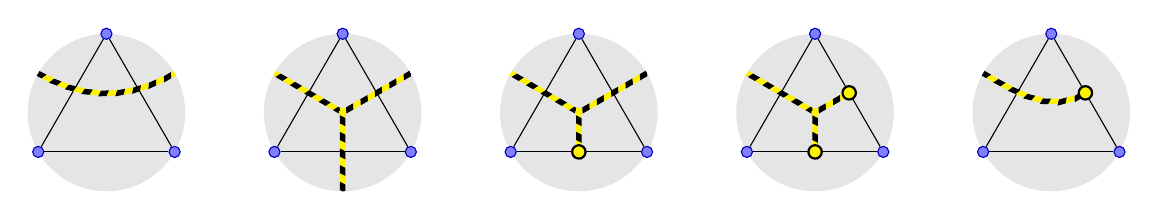
\begin{tikzpicture}[scale=1]
\begin{scope}[xshift=0cm]
	\path[fill=black!10] (0,0) circle (1);
	\node[marked] (1) at (90:1) {};
	\node[marked] (2) at (-30:1) {};
	\node[marked] (3) at (210:1) {};
	\draw (1) to node[below] {} (2);
	\draw (2) to node[below] {} (3);
	\draw (3) to node[below] {} (1);
	\clip (0,0) circle (1);
	\draw[barricade,out=210,in=-30] (30:1) to (150:1);
\end{scope}
\begin{scope}[xshift=3cm]
	\path[fill=black!10] (0,0) circle (1);
	\node[marked] (1) at (90:1) {};
	\node[marked] (2) at (-30:1) {};
	\node[marked] (3) at (210:1) {};
	\draw (1) to node[below] {} (2);
	\draw (2) to node[below] {} (3);
	\draw (3) to node[below] {} (1);
	\clip (0,0) circle (1);
	\draw[barricade] (150:1) to (0,0);
	\draw[barricade] (0,0) to (30:1);
	\draw[barricade] (0,0) to (270:1);
\end{scope}
\begin{scope}[xshift=6cm]
	\path[fill=black!10] (0,0) circle (1);
	\node[marked] (1) at (90:1) {};
	\node[marked] (2) at (-30:1) {};
	\node[marked] (3) at (210:1) {};
	\draw (1) to node[below] {} (2);
	\draw (2) to node[below] {} (3);
	\draw (3) to node[below] {} (1);
	\clip (0,0) circle (1);
	\draw[barricade] (150:1) to (0,0);
	\draw[barricade] (0,0) to (30:1);
	\draw[barricade] (0,0) to (270:.5);
	\node[barricade vertex] (b) at (270:.5) {};
\end{scope}
\begin{scope}[xshift=9cm]
	\path[fill=black!10] (0,0) circle (1);
	\node[marked] (1) at (90:1) {};
	\node[marked] (2) at (-30:1) {};
	\node[marked] (3) at (210:1) {};
	\draw (1) to node[below] {} (2);
	\draw (2) to node[below] {} (3);
	\draw (3) to node[below] {} (1);
	\clip (0,0) circle (1);
	\draw[barricade] (150:1) to (0,0);
	\draw[barricade] (0,0) to (30:.5);
	\draw[barricade] (0,0) to (270:.5);
	\node[barricade vertex] (a) at (30:.5) {};
	\node[barricade vertex] (b) at (270:.5) {};
\end{scope}
\begin{scope}[xshift=12cm]
	\path[fill=black!10] (0,0) circle (1);
	\node[marked] (1) at (90:1) {};
	\node[marked] (2) at (-30:1) {};
	\node[marked] (3) at (210:1) {};
	\draw (1) to node[below] {} (2);
	\draw (2) to node[below] {} (3);
	\draw (3) to node[below] {} (1);
	\clip (0,0) circle (1);
	\draw[barricade,out=210,in=-30] (30:.5) to (150:1);
	\node[barricade vertex] (a) at (30:.5) {};
\end{scope}
\end{tikzpicture}
\caption{Local pictures of barricades (up to rotation and reflection)}
\label{fig: local barricade}
\end{figure}

A \newword{short leaf}\margin[GM]{I can't decide if we want to allow non-short leaves in the definition. They make the proof of Prop. \ref{prop: inequalities} easier, but they don't appear in barricades related to the scattering diagram.} is a leaf whose adjacent vertex is in the adjacent triangle (e.g. the third and fourth local picture in Figure 
\ref{fig: local barricade}). A \newword{long leaf} is a leaf on the boundary of $\S$.

Barricades are considered up to isotopy within the set of barricades (so leaves must remain on arcs in $\Delta$). 
A measured lamination $\mu$ is \newword{compatible} with a barricade $B$ if there is are equivalent $\mu'$ and $B'$ such that $\mu'$ intersects $\Delta$ minimally and $\mu'$ and $B'$ do not intersect.%\margin[GM]{`Compatible' is a bit fiddly to define, since we need to be able to move the barricade around, but not 

\begin{prop}\label{prop: inequalities}
Given a barricade $B$, a measured lamination $\mu$ is compatible with $B$ iff the following inequalities hold.
\begin{itemize}
	\item For each path in $B$ which begins with a right turn and ends with a left turn,
	\[ S_{1}(\mu) + S_{2}(\mu) + ... + S_{n}(\mu) \geq 0\]
	where $S_1, S_2,...,S_n$ are the shear coordinates of the arcs in $\Delta$ crossed by $P$.
	\item For each path in $B$ which begins with a left turn and ends with a right turn, 
	\[ S_{1}(\mu) + S_{2}(\mu) + ... + S_{n}(\mu) \leq 0\]
	where $S_1, S_2,...,S_n$ are the shear coordinates of the arcs in $\Delta$ crossed by $P$.
	\item For each cycle in $B$, 
	\[ S_{1}(\mu) + S_{2}(\mu) + ... + S_{n}(\mu) = 0\]
	where $S_1, S_2,...,S_n$ are the shear coordinates of the arcs in $\Delta$ crossed by $P$.
\end{itemize}
\end{prop}

%Given a barricade $B$, let $C_B\subset \mathbb{R}^\Delta$ be the set of measured laminations which are compatible with $B$.

\begin{corollary}
Given a barricade $B$, the set $C_B\subset \mathbb{R}^\Delta$ of measured laminations which are compatible with $B$ is a closed cone. 
\end{corollary}



%\begin{definition}
%Given an (ordinary, untagged) triangulation $\Delta$ of $(\S,\M)$, an \newword{I-beam} is a graph $I$ embedded in $\S$, such that, when restricted to the neighborhood of a triangle in $\Delta$, the connected components are isotopic to one of pictures in Figure \ref{fig: local I-beams}.
%\end{definition}

%\begin{figure}[h!t]
%\begin{tikzpicture}[scale=1]
%\begin{scope}[xshift=0cm]
%	\draw[fill=black!10, dashed] (0,0) circle (1);
%	\node[marked] (1) at (90:1) {};
%	\node[marked] (2) at (-30:1) {};
%	\node[marked] (3) at (210:1) {};
%	\draw (1) to node[below] {} (2);
%	\draw (2) to node[below] {} (3);
%	\draw (3) to node[below] {} (1);
%	\draw[red,out=210,in=-30] (30:1) to (150:1);
%\end{scope}
%\begin{scope}[xshift=3cm]
%	\draw[fill=black!10, dashed] (0,0) circle (1);
%	\node[marked] (1) at (90:1) {};
%	\node[marked] (2) at (-30:1) {};
%	\node[marked] (3) at (210:1) {};
%	\draw (1) to node[below] {} (2);
%	\draw (2) to node[below] {} (3);
%	\draw (3) to node[below] {} (1);
%	\node[inner sep=0.5mm,circle,draw=red] (a) at (30:.5) {};
%	\node[inner sep=0.5mm,circle,draw=red] (b) at (270:.5) {};
%	\draw[red] (150:1) to (0,0);
%	\draw[red] (0,0) to (a);
%	\draw[red] (0,0) to (b);
%\end{scope}
%%\begin{scope}[xshift=6cm]
%%	\draw[fill=black!10, dashed] (0,0) circle (1);
%%	\node[marked] (1) at (90:1) {};
%%	\node[marked] (2) at (270:1) {};
%%	\node[marked] (3) at (0,0) {};
%%	\draw[out=-15,in=15] (1) to (2);
%%	\draw[out=195,in=165] (1) to (2);
%%	\draw[out=-60,in=60] (1) to (3);
%%	\draw[out=-120,in=120] (1) to (3);
%%	\draw[red] (3) to (0,-.5);
%%	\draw[red,out=-30,in=210] (0,.-.5) to (0:1);
%%	\draw[red,out=210,in=-30] (0,.-.5) to (180:1);
%%\end{scope}
%%\begin{scope}[xshift=9cm]
%%	\draw[fill=black!10, dashed] (0,0) circle (1);
%%	\node[marked] (1) at (90:1) {};
%%	\node[marked] (2) at (270:1) {};
%%	\node[marked] (3) at (0,0) {};
%%	\draw[out=-15,in=15] (1) to (2);
%%	\draw[out=195,in=165] (1) to (2);
%%	\draw[out=-60,in=60] (1) to (3);
%%	\draw[out=-120,in=120] (1) to (3);
%%	\draw[red] (3) to (0,-.5);
%%	\draw[red,out=-30,in=210] (0,.-.5) to (0:1);
%%	\draw[red,out=210,in=-30] (0,.-.5) to (180:1);
%%\end{scope}
%\end{tikzpicture}
%\caption{Local pictures of I-beams (no punctures)}
%\label{fig: local I-beams}
%\end{figure}



%\begin{thm}
%The scattering diagram of $(\S,\M)$ in $\mathbb{R}^\Delta$ has a wall for each minimal barricade of codimension $1$ (supported on the compatible cone), and a joint for each minimal barricade of codimension $2$ (supported on the compatible cone).
%\end{thm}

%\begin{ex}
%
%Consider the following barricade.
%
%\begin{center}
%\begin{tikzpicture}
%\begin{scope}[scale=.5]
%	\draw[fill=black!10] (0,0) circle (2);
%	\node[marked] (1) at (90:2) {};
%	\node[marked] (2) at (18:2) {};
%	\node[marked] (3) at (306:2) {};
%	\node[marked] (4) at (234:2) {};
%	\node[marked] (5) at (162:2) {};	
%%	\draw (1) to (2);
%%	\draw (2) to (3);
%%	\draw (3) to (4);
%%	\draw (4) to (5);
%%	\draw (5) to (1);
%	\draw (1) to (3);
%	\draw (1) to (4);
%	\draw[barricade] (54:2) to (-78:2);
%	
%\end{scope}
%\end{tikzpicture}
%\end{center}
%
%\end{ex}

%\newpage

\section{Proof of Proposition \ref{prop: inequalities}}

Let us collectively refer to the inequalities in Proposition \ref{prop: inequalities} as the \newword{compatibility inequalities} for $B$ and $\mu$. 

A barricade is \newword{simple} if it is connected and has no degree $3$ vertices. We start by proving a stronger version of Proposition \ref{prop: inequalities} in the case of a simple barricades.

\begin{lemma}\label{lemma: simplebarricade}
Let $B$ be a simple barricade in $\Delta$. A measured lamination $\mu$ is compatible with $B$ iff it satisfies the compatibility inequalities.
\end{lemma}

\begin{proof}[Proof idea]
Induction, I hope. I don't know about loops, though.
\end{proof}
	
\begin{lemma}\label{lemma: simplesub}
A measured lamination $\mu$ is compatible with a barricade $B$ iff $\mu$ is compatible with every simple sub-barricade of $B$.
\end{lemma}

\begin{proof}[Proof idea]
If they are incompatible, there should be some unmarked curve that is crossed.
\end{proof}

\begin{proof}[Proof of Proposition \ref{prop: inequalities}]
Assume $\mu$ is compatible with $B$. For any path or cycle in $B$, there is a simple sub-barricade $B'$ containing that path or cycle which is also compatible with $\mu$, and so the associated compatibility inequality holds by Lemma \ref{lemma: simplebarricade}.

Assume the compatibility inequalities hold for $\mu$ and $B$. Then they also hold for any simple sub-barricade of $B$, and so by Lemma \ref{lemma: simplebarricade} $\mu$ is compatible with each of them. By Lemma \ref{lemma: simplesub}, $\mu$ is compatible with $B$.
\end{proof}

\section{Minimal barricades}

%\begin{prop}
%If a measured lamination $\mu$ is compatible with a barricade $B$, 
%\end{prop}

\begin{definition}
The \newword{codimension} of a barricade is the codimension of (the span of) the compatible cone. A barricade is \newword{minimal} if it has no sub-barricades of the same codimension.
\end{definition}

Easy observation: all leaves in a minimal barricade are short, since they can be cut off without increasing the codimension.

%If $B$ has no loops, the span of the compatible cone has codimension equal to the number of edges in $B$ whose endpoints are degree $3$ vertices.



\begin{conj}
The codimension of a barricade $B$ is 
\[ (\text{$\#$ of edges between trivalent vertices}) + (\text{$\#$ of loops without leaves}) \]
\end{conj}

\begin{corollary}
The minimal barricades of codimension $1$ are:
\begin{itemize}
	\item Trees with $4$ leaves, all short.
	%which are locally isomorphic to the pictures in Figure \ref{fig: local I-beams}.
	\item A cycle with $0$ leaves.
\end{itemize}
\end{corollary}

\begin{corollary}
The minimal barricades of codimension $2$ are:
\begin{itemize}
	\item Trees with $5$ leaves, all short.
	\item A cycle with $2$ leaves, all short.
	\item Disjoint unions of $2$ minimal barricades of codimension $1$.
\end{itemize}
\end{corollary}

\begin{lemma}
If $B$ and $B'$ are minimal barricades, then 
\[ C_B\cap C_{B'} = \bigcup _i C_{B_i} \]
where each of the $B_i$ are minimal barricades. 
\end{lemma}

%\begin{conj}
%The codimension of a barricade $B$ is 
%\begin{align*}
%&\frac{3(\text{$\#$ of branches}) - \text{$\#$ of leaves}}{2} + (\text{$\#$ of components without branches})
%%\#&\text{ of edges in $B$ with a branch at each endpoint} \\
%%&+ \#\text{ of loops (i.e. cycles without branches)} \\
%%&+ \text{total genus of components of $\S\smallsetminus B$ that don't contain marked points}\\
%\end{align*}
%\end{conj}

\section{The scattering diagram of $(\S,\M)$}

We fix a triangulation $\Delta$ of $(\S,\M)$, and we use the language of barricades to construct a scattering diagram in $\mathbb{R}^\Delta$. We distinguish two kinds of minimal barricades of codimension $1$.
Construct a scattering diagram $\mathfrak{D}$ in $\mathbb{R}^\Delta$ as follows.
\begin{itemize}
	\item A \newword{I-beam} is a tree with $4$ short leaves. For each {I-beam} $B$, $\mathfrak{D}$ has a wall
	\[ (C_B, 1+x^{\mathsf{B}n} )\]
	where $n\in\mathbb{N}^\Delta$ counts the transverse crossings of $B$ and the arcs in $\Delta$.
	\item A \newword{non-shielding loop} is a cycle with $0$ leaves, such that each component of the complement contains a marked point. For each {non-shielding loop} $B$, $\mathfrak{D}$ has a wall
	\[ \left(C_B, (1-x^{\mathsf{B}n})^{-2} \right)\]
	where $n\in\mathbb{N}^\Delta$ counts the transverse crossings of $B$ and the arcs in $\Delta$.
\end{itemize}

\begin{theorem}\label{thm: consistent}
The scattering diagram $\mathfrak{D}$ is consistent, and is the GHKK scattering diagram of the seed $\Delta$ in the cluster algebra associated to $(\S,\M)$.
\end{theorem}

\subsection{Proof of Theorem \ref{thm: consistent}}

\begin{lemma}
The joints of $\mathfrak{D}$ are as follows.%are $C_B$, as $B$ runs over the minimal barricades of codimension $2$.
\begin{itemize}
	\item If $B$ is a tree with 5 short leaves, then $C_B$ is a joint which is contained in the 3 walls; specifically, the 3 I-beams contained in $B$.
	\item If $B$ is a cycle with 2 short leaves on the same side, then $C_B$ is a joint which is contained in 2 or 3 walls; specifically, the 2 I-beams contained in $B$, and the cycle (if it is non-shielding).
	\item If $B$ is a cycle with 2 short leaves on different sides, then $C_B$ is a joint which is contained in infinitely many walls; specifically, the infinitely-many I-beams contained in $B$, and the cycle.\footnote{Note that the cycle in this case must be non-shielding.}
	\item If $B$ is a disjoint union of $2$ I-beams or non-shielding loops, then $C_B$ is a joint contained in 2 walls.
\end{itemize}
\end{lemma}

\begin{thebibliography}{27}

\bibitem{cats1}
S. Fomin, M. Shapiro, and D. Thurston,
\textit{Cluster algebras and triangulated surfaces. I. Cluster complexes.}
Acta Math. \textbf{201} (2008), no. 1, 83--146. 

\bibitem{cats2}
S. Fomin and D. Thurston,
\textit{Cluster algebras and triangulated surfaces. Part II: Lambda lengths.}
Preprint, 2008.
(arXiv:1210.5569)

\bibitem{GHK}
M. Gross, P. Hacking, and S. Keel,
\textit{Birational geometry of cluster algebras.}
Algebraic Geometry \textbf{2} (2015) 137--175.

\bibitem{GHKK}
M. Gross, P. Hacking, S. Keel, and M. Kontsevich,
\textit{Canonical bases for cluster algebras.}
Preprint, 2014. \texttt{arXiv:1411.1394}

\bibitem{unisurface}
N. Reading,
\textit{Universal geometric cluster algebras from surfaces. }
Trans. Amer. Math. Soc. \textbf{366} no. 12 (2014), 6647--6685.

\bibitem{scatfan}
N. Reading, 
\textit{Scattering fans}. 
In preparation.

\bibitem{dominance}
N. Reading, 
\textit{Dominance phenomena: Mutation, scattering and cluster algebras}. 
In preparation.

\end{thebibliography}


\end{document}  